\documentclass[conference]{IEEEtran}
\IEEEoverridecommandlockouts

% Required packages from IEEE template
\usepackage{cite}
\usepackage{amsmath,amssymb,amsfonts}
\usepackage{graphicx}
\usepackage{textcomp}
\usepackage{xcolor}

% Additional packages from original ACM paper
\usepackage{tikz}
\usepackage{filecontents}
\usepackage{xspace}
\usepackage{threeparttable}
\usepackage{makecell}
\usepackage{url}
\usepackage{soul}
\usepackage{colortbl}
\usepackage{multirow}
\usepackage{tabularx}
\usepackage{pifont, mathtools}
\usepackage[overload]{empheq}
\usepackage{nccmath}
\usepackage{cases}
\usepackage{float}
\usepackage{subcaption}
\usepackage{adjustbox}
\usepackage{booktabs}
\usepackage{comment}
\usepackage[normalem]{ulem}
\usepackage{enumitem}
\usepackage{listings}
\usepackage{color}
\usepackage{balance}
\usepackage{caption}

% Font settings
\usepackage{pifont}
\newcommand{\xmark}{\ding{55}}
% \usepackage[font=small]{caption}
% \captionsetup[figure]{font=small}
% \captionsetup[table]{font=small}

\captionsetup{font=footnotesize}

% Custom commands
\newcommand{\para}[1]{\noindent {\bf #1}}
\newcommand{\vnsdi}[1]{{\color{blue} #1}}
\definecolor{red}{rgb}{1,0,0}
\definecolor{gray}{rgb}{0.5,0.5,0.5}
\newcommand{\yc}[1]{{\color{red} #1}}
\newcommand{\hxq}[1]{{\color{red}hx: #1}}
\newcommand{\hx}[1]{{\color{red} #1}}
\newcommand{\fyc}[1]{{\color{black} #1}}
\newcommand{\jz}[1]{{\color{purple} #1}}
\newcommand{\todo}[1]{\textbf{\color{gray}{#1}}}
% \newcommand{\fx}[1]{{\color{orange!90!black}{#1}}}

\newcommand{\fx}[1]{{\color{black} #1}}


% Hyperref and cleveref
\usepackage{hyperref}
\hypersetup{colorlinks={true},linkcolor={violet},citecolor=blue}
\usepackage{cleveref}
\Crefname{appendix}{Appendix}{Appendices}
\crefname{appendix}{appendix}{appendices}
\crefname{section}{}{\S\S}
\crefdefaultlabelformat{\S#2#1#3}

%%%%%%%%%%%%%%%%%%%% global vars %%%%%%%%%%%%%%%%%%%%
\newcommand\hmm[1]{\ifnum\ifhmode\spacefactor\else2000\fi>1000 \uppercase{#1}\else#1\fi}
\newcommand{\sys}{Moye\xspace}
\newcommand{\bs}{Proteus\xspace}
\newcommand{\ff}{FlexFlow\xspace}

\newcommand{\op}{operation\xspace}
\newcommand{\ops}{operations\xspace}
\newcommand{\Op}{Operation\xspace}
\newcommand{\Ops}{Operations\xspace}

\newcommand{\wg}{\hmm{e}xecution graph\xspace}
\newcommand{\Ep}{Ex-situ simulation\xspace}
\newcommand{\ep}{ex-situ simulation\xspace}

\newcommand{\extractor}{\hmm{w}orkload tracer\xspace}
\newcommand{\cm}{CC estimator\xspace}
\newcommand{\ma}{\hmm{t}imeline composer\xspace}
\newcommand{\va}{\hmm{v}alidator\xspace}
\newcommand{\nccl}{NCCL\xspace}
\newcommand{\bd}{\texttt{broadcast}\xspace}
\newcommand{\ar}{\texttt{all-reduce}\xspace}
\newcommand{\ag}{\texttt{all-gather}\xspace}
\newcommand{\rs}{\texttt{reduce-scatter}\xspace}
\newcommand{\send}{\texttt{send}\xspace}
\newcommand{\recv}{\texttt{receive}\xspace}
\newcommand{\rd}{\texttt{reduce}\xspace}
%%%%%%%%%%%%%%%%%%%%%%%%%%%%%%%%%%%%%%%%%%%%%%%%%%%%%%

\def\BibTeX{{\rm B\kern-.05em{\sc i\kern-.025em b}\kern-.08em
    T\kern-.1667em\lower.7ex\hbox{E}\kern-.125emX}}

\begin{document}

%%%%%%%%%%%%%%%%%%%%%%%%%%%%%%%%%%%%%%%%%%%%%%%%%%
% ANONYMIZED VERSION FOR BLIND REVIEW
% Author information has been removed
%%%%%%%%%%%%%%%%%%%%%%%%%%%%%%%%%%%%%%%%%%%%%%%%%%
\title{Scalable and Efficient Simulation of LLM Training}

% % Anonymized author block - DO NOT REMOVE for blind review
% \author{\IEEEauthorblockN{Anonymous Submission}
% \IEEEauthorblockA{Paper ID: XXXX}}

\maketitle

%!TEX root = main.tex

\begin{abstract}

Simulation offers unique values for both enumeration and extrapolation purposes, and is becoming increasingly important for managing the massive machine learning (ML) clusters and large-scale distributed training jobs.
In this paper, we build \sys to tackle three key challenges in large-scale training simulation:
(1) tracing the runtime training workloads at each device in an ex-situ fashion so we can use a single device to obtain the actual execution graphs of 1K-GPU training, (2) accurately estimating the collective communication without high overheads of discrete-event based network simulation, and (3) accounting for the interference-induced computation slowdown from overlapping communication and computation kernels on the same device.
\sys supports both dense and MoE workloads with high fidelity and further enables GPU memory–aware ex-situ simulation. 
\sys delivers on average 8\% error in training step---$\sim$3x lower than state-of-the-art simulators---for GPT-175B on a 96-GPU H800 cluster with 3D parallelism on Megatron-LM under 2 minutes.
% On a 96-GPU H800 cluster, \sys achieves an average step-time error of 8\% for GPT-175B with 3D parallelism on Megatron-LM, delivering $\sim$3$\times$ lower error than state-of-the-art simulators, all within 2 minutes.  
% It can simulate a 8,192-GPU setting in 1.38 hours compared to 5.2 days for recent work using ns-3. 
% The scaling law have made it standard practice to train large-scale deep neural network (DNN) models using thousands of GPUs, leveraging state-of-the-art techniques. This approach necessitates a precise simulator to assist with the design and optimization of the training process before actual model training begins, significantly reducing both time and financial costs throughout the development pipeline. However, existing simulators fail to meet these demands due to their inability to accurately model computation and communication workloads in large-scale training scenarios.
% In this paper, we re-examine existing simulation approaches and, based on this analysis, introduce our simulator, Moye. To closely replicate the training process, we delve into mainstream training frameworks and communication libraries, developing a suite of tools that facilitate accurate construction of training workloads, prediction of communication times, and simulation of performance slowdowns caused by kernel overlap. We adopt a profile-and-predict approach to derive the iteration time of large-scale distributed tasks from knowledge obtained from small-scale tasks. We evaluate the performance of the simulator on NVIDIA H800 and A800 clusters, demonstrating an average prediction accuracy of up to 92.25\%.




\end{abstract}


% Keywords are commented out per user requirement
% \begin{IEEEkeywords}
% Large Language Models, Training Simulation, Distributed Systems
% \end{IEEEkeywords}

%!TEX root = main.tex 

\section{Introduction} 
\label{sec:introduction}
% % scaling phnomenone
% Recently, we have witnessed wide success and great potential in deep neural networks (DNNs). With the growing size of DNN models~\cite{shoeybi2019megatron, lepikhin2020gshard} and datasets, LLM training has become a standard practice to meet the computation requirements. Compared with single-device training, LLM training using multiple devices can substantially improve training throughput. The cluster size of LLM training increases rapidly \cite{goyal2017accurate}.


%%%%%%%%%%%%%%%%%%%%%%%%%%%%%%%%%%%%%%%%%%%%%%%%%%%%% new version %%%%%%%%%%%%%%%%%%%%%%%%%%%%%%%%%%%%%%%%%%%%%%%%%%%%%
% scaling phnomenone
The unprecedented success of large language models (LLMs) has been driven in large part by the large-scale infrastructures that allow the model and training dataset to scale. 
Organizations have constructed massive clusters with tens of thousands of GPUs to train models with hundreds of billions or even trillions of parameters~\cite{jiang2024megascale,goyal2017accurate,llama3-meta}, in a continuous stride to improve model capabilities.
%  as promised by the scaling law~\cite{kaplan2020scaling}.

% The scaling law underscores that the size of a deep neural network (DNN) model and its training data are pivotal in determining the model's capability~\cite{jiang2024megascale}. To achieve state-of-the-art (SOTA) performance, leading  
% For instance, OpenAI and Meta use over 15,000 advanced GPUs to train their large language models (LLMs)~\cite{jiang2024preventing,llama3-meta}.

% why we need a simulator: enumeration and extrapolation
% 1. search for optimal training plan
% 2. extrapolate gains of new hardware/strategy for planning
Training LLMs on such massive scales consumes substantial time and financial resources. It is also inherently complex and rapidly evolving with a myriad of algorithm/model innovations~\cite{katharopoulos2020transformers,SMMD17}, parallelism strategies~\cite{zhao2023pytorch,ren2021zero,liu2024deepseek}, kernel optimization (\cite{SBZT24,dao2022flashattention}), and hardware designs \cite{memryx}. 
% parallelism strategies and optimization techniques across the entire stack of from software to hardware to maximize the utilization of cluster resources.
% algorithm-level innovation, op-level parallelism, op-level algorithm
% \fx{The complexity is further compounded by emerging architectures like Mixture-of-Experts (MoE)}~\cite{liu2024deepseek,dai2024deepseekmoe}. HX:already mentioned in model innovations
As a result, accurate simulation of LLM training has started to garner attention as an essential building block to effectively manage training infrastructures and systems~\cite{SimAI2025NSDI,duan2024proteus,won2023astra,lu2023distsim,hu2022dpro}. 

Broadly, simulation is useful for two main purposes: enumeration and extrapolation.
In LLM training context, simulation can be used to enumerate combinations of parallelism strategies, optimization techniques, and hardware configurations that are available in the current cluster, to derive the optimal training plan for a given job and to determine efficient resource allocation schedules across jobs \cite{SimAI2025NSDI,duan2024proteus}.
Simulation is also useful (perhaps more so) to extrapolate beyond the currently available resources, which is paramount for strategic decision making such as capacity planning~\cite{jiang2024megascale,shoeybi2019megatron} that involve what-if questions with significant impact.
For example, what speed-up can be expected by scaling the current cluster by a factor of 5, or by increasing the network bandwidth by 2x?
This also greatly facilitates the development of new optimizations, which only need to be prototyped on a small scale for the simulator to extrapolate its potential benefits on a much larger scale.


Prior work has made salient progress on training simulation~\cite{jia2019beyond,zhu2020daydream,hu2022dpro,lu2023distsim,isaev2023calculon,won2023astra,liang2025lumos,SimAI2025NSDI,duan2024proteus}. 
Yet, they fall short in three key aspects that hinder their capabilities in supporting both enumeration and extrapolation practically.

% First, modern large-scale training often employs 3D parallelism, a combination of data parallelism (DP), tensor parallelism (TP), and pipeline parallelism (PP), to break down the large models along different dimensions into sub-models that fit into a device's memory and maximize cluster resource utilization.
First, LLM training employs {data parallelism (DP), tensor parallelism (TP), pipeline parallelism (PP), and expert parallelism (EP) for MoE models}, to break up a large model along different dimensions.
To accurately simulate {various parallelism strategies and their memory usages on each device}, one needs to obtain the training workloads, which encompass the device- or rank-specific execution graphs {detailing the computation, communication, and memory events, along with their dependencies.}
Existing work \cite{hu2022dpro,lu2023distsim,luo2022srifty,zhu2020daydream,SimAI2025NSDI} requires a full-scale cluster deployment of the job to trace the training workloads from each and every device at runtime.
This is because each device builds its own execution graph independently in parallel during job initialization to most efficiently carry out training of its unique sub-model.
%  according to the parallelism strategy setting and various optimization techniques (e.g. kernel fusion).
%  perform runtime tracing at each device to collect training workloads.
The \textit{in-situ} tracing approach is clearly very costly and sometimes even impractical for extrapolation usecases.
% \fx{Ensuring these complex configurations truly "fit" requires accurately predicting peak GPU memory in training. Practitioners often resort to overly conservative memory estimates to preempt unexpected and costly out-of-memory (OOM) errors. This strategy, however, can lead to significant under-utilization of GPU resources.
% % , causing them to miss more optimal training configurations (see Section~\ref{sec:usecase}).
% }


% exisiting simualtor and why they cannot work
% Existing simulators, however, are not well-suited for large-scale scenarios (a detailed comparison of their formulation capabilities is provided in Table~\ref{tab:work_compare}). These simulators primarily fall into two categories. The first category is realism-oriented, where tools like Habitat~\cite{geoffrey2021habitat} rely on hardware metrics~\cite{kothapalli2009performance,zhang2011quantitative,liu2021seer} or learning-based models~\cite{chen2018tvm,baghdadi2021deep} but are confined to single-GPU scenarios. Multi-GPU simulators, such as Daydream~\cite{zhu2020daydream}, Srift~\cite{luo2022srifty} and dPRO~\cite{hu2022dpro}, focus only on data parallelism and depend heavily on specific hardware setups and datasets, limiting their scalability. While DistSim~\cite{lu2023distsim}, ASTRA-sim~\cite{won2023astra} and Proteus~\cite{duan2024proteus} attempt to simulate complex large-scale training, they fail to accurately capture training workloads and oversimplify communication modeling. SimAI~\cite{SimAI2025NSDI} introduces a unified simulator, but it overlooks the potential complexities of training behavior, and its reliance on costly, hacky solutions makes extension and maintenance  challenging.
% The second category is optimization-oriented. FlexFlow~\cite{jia2019beyond}, for example, customizes a simulator to explore parallelization strategies, but approaches~\cite{fan2021dapple,elango2021pase} like this lack programmability and are limited to optimizing parallelism rather than accurately replaying the training process~\cite{duan2024proteus}.


% challenges
% Thus, there is an urgent need for a scalable and precise simulator to address the complex requirements of large-scale DNN training. Through our practice, we identified three main challenges that must be overcome.


%%  challenges 2
{Second}, simulating collective communication (CC) is critical because (1) it pieces all the devices and nodes together according to the parallelisms, and (2) its performance can often be the bottleneck \cite{duan2024efficient, qi2023zero, jiang2024megascale, huang2019gpipe}. 
% Each training iteration involves numerous communication operations (e.g., All-Reduce, All-Gather), which support various parallel training strategies and consume a significant portion of time in large-scale LLM training.
Most existing work~\cite{duan2024proteus, won2023astra,hu2022dpro,lu2023distsim,zhu2020daydream} rely on a coarse-grained $\alpha$-$\beta$ model \cite{valiant1990bridging} to simulate the CC time without considering the actual communication patterns and implementation optimizations.
% , resulting in significant simulation errors.  
On the other hand, more recent work such as SimAI \cite{SimAI2025NSDI} explicitly simulates each peer-to-peer (P2P) send and receive primitive of a CC kernel using a packet-level event-based network simulator such as ns-3 \cite{riley2010ns}.
This fine-grained approach provides high accuracy at the cost of prohibitive overheads even at a medium scale: simulating a 128-GPU job takes SimAI over 2 hours with an optimized ns-3 implementation (\cref{subsec:challenges}). 

%%  challenges 3
{Third}, overlapping communication and computation \ops, an optimization widely used to improve efficiency \cite{chang2024flux, jiang2024megascale,chen2024centauri,zhang2017poseidon}, incurs non-negligible slowdowns to the computation due to contention for shared resources (e.g., cache, DRAM bandwidth) \cite{hwang2023ark,duan2024proteus}.
% complex kernel behaviors emerge when employing SOTA training techniques, potentially impacting simulation accuracy.
% A common optimization is the concurrent execution of computation and communication kernels to improve performance~. However, this concurrency often introduces additional slowdown effects (details provided in §\ref{subsec:challenges2}) due to GPU resource contention~.
This, however, has largely been overlook thus far.
Simulating interference-induced slowdown is particularly challenging since it depends on many idiosyncrasies ranging from scheduling logic of the ML framework and the underlying library to hardware-specific implementation optimizations.
Much of these details are vendor-proprietary and inaccessible. 
% These slowdown factors are highly dynamic and influenced by various factors, including the hardware and software environment during kernel execution, making them difficult to capture.


% our work
% In this work, we propose \sys, a dedicated simulator for large-scale distributed DNN training. Our design and implementation span the entire stack, leveraging mainstream training frameworks and communication libraries. Our key idea is to generate training workloads by extracting critical simulation information directly from the dataflows of these frameworks and libraries by enabling a special runtime mode, and to supplement the remaining simulation components (e.g., commnunication kernel running time and overlap slowdown factors) using a reasonable predictive approach, and in the end, reoraganize all execution operators to global timelines properbly based on domain-knowlege which pre-defined in simulator.

In this work, we build \sys, a practical simulation platform for large-scale LLM training. 
\sys is built with three key design choices.
(1) It adopts an \textit{ex-situ} tracing approach to accurately capture training workloads using just a single device, avoiding the need for a full-scale cluster deployment. The key technical idea here is to transform the parallel initialization process at each rank into a sequential one, allowing a single device to act as each rank iteratively to trace the corresponding execution graph and GPU memory footprints.
(2) It employs white-box modeling to simulate a CC kernel's performance with four parts: connection setup overhead, intra-server and inter-server transmission, and possible data reduction time. 
% , and  as a series send and receive primitives according to the algorithms (ring vs tree). 
The model is supplemented with exhaustive profiling to obtain key parameters (e.g. chunk size which determines number of rounds of transmission for a message) optimized by CC libraries like \nccl for different hardware features and software configurations that affect the individual components above.
This hybrid approach strikes a good balance between accuracy and efficiency.
(3) It introduces an black-box ML-based slowdown predictor to model the slowdown caused by overlapping \ops. 
The XGBoost-based predictor relies on categorical features such as transmission protocol and channel configuration in \nccl, to numerical kernel-level performance statistics such as streaming multiprocessors (SM) occupancy and DRAM utilization, to capture their complex interactions.
%  the slowdown factor in LLM training.

% (3) It introduces an ML-based slowdown predictor to model the interference between overlapping computation and communication kernels.
% Our design and implementation encompass the entire stack, leveraging mainstream training frameworks and communication libraries. Our key idea is to generate accurate training workloads by extracting critical simulation information directly from the dataflows of these frameworks and libraries through a specialized runtime mode. To complement this, we employs tailored predictive approaches in \sys to model missing simulation components, such as communication kernel runtime and overlap-induced slowdown factors. Finally, we reorganizes all execution operators into global timelines based on domain knowledge pre-defined within the simulator.

We implement \sys to support mainstream training frameworks: PyTorch,  DeepSpeed~\cite{rasley2020deepspeed}, and Megatron-LM~\cite{shoeybi2019megatron}.
Our implementation with $\sim$10k LoC also includes a suite of automation tools to facilitate workload tracing and runtime profiling.
We evaluate \sys on H800 and A800 clusters across a variety of scenarios and models, achieving an average prediction accuracy of 91.4\% in training step time, and is up to 3x better than the state-of-the-art. 
% \hxq{comp. and comm. results?}
For 96-GPU training of GPT-175B, \sys achieves 92\% accuracy in less than 2 minutes. 
Beyond dense models, \sys provides high-fidelity support for MoE workloads (average error 3.4\%) and further enables GPU memory–aware ex-situ simulation. 
We plan to open source \sys to the community.
% \hxq{revise this to reflect the new changes}
% \jz{(Consider adding exp data to compare Moye with baselines.)} To reduce simulation overhead, \sys leverages a reusable database of profiling statistics. Simulating a 175B GPT model on a 256-GPU cluster takes less than 3 minutes.



%% challeneg2
% To address the second challenge, we analyze chunk-level data propagation mechanism within the NVIDIA Collective Communications Library (NCCL)~\cite{nccl} and propose a runtime model that considers intra-server and inter-server delays, data reduction operations, and connection setup overhead. We profile these factors on a small-scale cluster and use them to simulate the target configuration.

%% challeneg3
% To tackle the third challenge, we adopt a black-box approach utilizing a machine learning (ML) model. This model learns resource contention between concurrent kernels using kernel-level performance statistics from single-device training, along with training configurations, to estimate the slowdown factor in LLM training.

% experiments

% In §\ref{sec:evaluation}, we also demonstrate \sys's ability to assist engineers in optimizing the training process by providing detailed reports on load balancing, synchronization times, parameter sizes across different communication parallel groups, and more.

% contributions
% In summary, our contributions are the following:
% \begin{itemize}[leftmargin=2mm]
%     \item We develop a profiling toolkit that intercepts and overrides requests from the training framework, enabling precise and automated workload capture on a single host while circumventing hardware constraints. This toolkit  captures operators and manages complex dependencies under SOTA parallel strategies scenario.
%     \item We conduct an in-depth analysis of the internal mechanism of NCCL and design a communication estimator using a hybrid profiling and formulation approach. This allows us to accurately predict large-scale communication performance from small-scale cluster measurements.
%     \item We conduct extensive experiments on the concurrent execution of communication and computation kernels. We analyze the potential factors that are critical to resource contention and propose an ML-based predictor to simulate the interference and predict the slowdown factor.
%     \item We design and implement the simulator for PyTorch, DeepSpeed, and Megatron-LM. It adopts a profile-and-predict approach to estimate training performance. We validate it on large-scale training clusters and large models. We plan to open-source the simulator and profiling database.
% \end{itemize} 


%!TEX root = main.tex 

\section{Background and Motivation} 
\label{sec:motivation} 

\subsection{Large-scale LLM Training} 
\label{subsec:background}



% Advancements in infrastructure have dramatically increased the scale and complexity of modern AI training. 
\noindent Figure~\ref{fig:tech_overview} illustrates the layered technical stack underlying LLM training, from high-level models and frameworks to low-level GPU libraries and networked systems. 
% Today's LLMs often exceed 100 billion parameters~\cite{jiang2024preventing,llama3-meta}, and recent GPU architectures (e.g., NVIDIA Hopper and Ampere) combined with high-speed interconnects (e.g., InfiniBand and RoCE) enable efficient training at the scale of thousands of GPUs. Parallelism strategies with communication-computation overlap \cite{liu2024deepseek} further improve utilization and accelerate training.

\begin{figure}[t]
    \centering 
    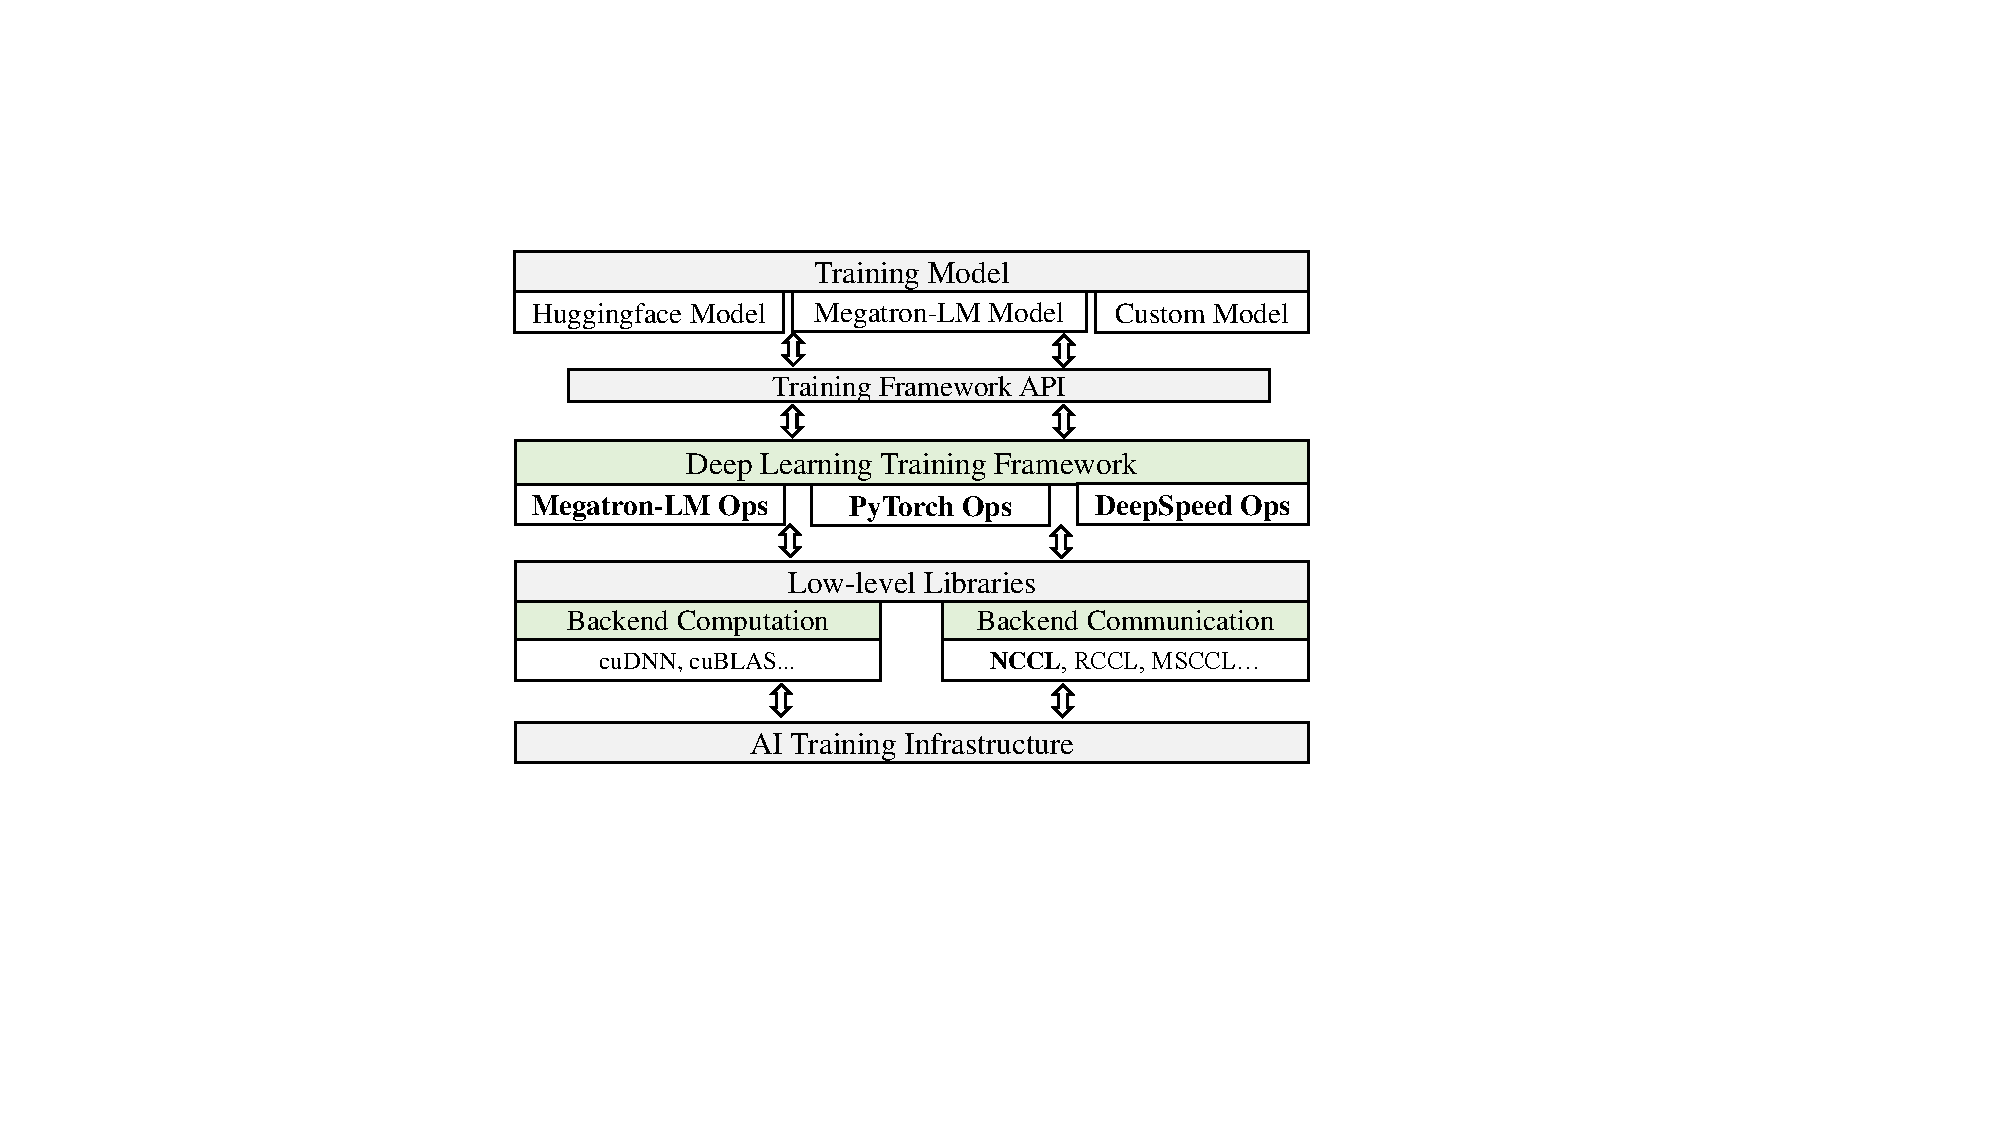
\includegraphics[width=0.9\linewidth]{figures/motivation/tech_overview.pdf} 
    \vspace{-1mm}
    \caption{Overview of the technical stack for LLM training.} 
    \label{fig:tech_overview}
    \vspace{-1.5mm}
\end{figure}
% \noindent\textbf{Training frameworks.} 
LLM training jobs are executed on frameworks such as Megatron-LM~\cite{shoeybi2019megatron} and PyTorch~\cite{rasley2020deepspeed,shoeybi2019megatron,SimAI2025NSDI}. They implement parallelism strategies combining DP, TP, PP, and EP to efficiently scale model training across large GPU clusters. 
Chiefly, DP replicates the model and splits the data, TP divides model parameters among GPUs, PP stages model layers for pipelined execution, while EP distributes experts of a MoE model across devices.
% Together, these methods accelerate training of hundred-billion-parameter models. 
% \noindent\textbf{Communication library.} 
Collective Communication Libraries (CCLs) then facilitate data transfer across ranks. NCCL is the de-facto CCL in production~\cite{weingram2023xccl,shoeybi2019megatron,SimAI2025NSDI,rasley2020deepspeed}.
% , including advanced topological algorithms and protocols that decompose data transmission into efficient P2P transfers.
\begin{table*}[t]
    \centering
    \small
    \setlength{\tabcolsep}{2.5pt}
    \renewcommand{\arraystretch}{0.95}
    \begin{tabular}{@{}cccccccc@{}}
    \toprule

    \multirow{2}{*}[-5pt]{Simulator} & 
    \multicolumn{3}{c}{Training Workload} & 
    \multirow{2}{*}[-5pt]{\makecell{3D Parallelism}} & 
    \multirow{2}{*}[-5pt]{\makecell{MoE/EP \\ Support}} & 
    \multirow{2}{*}[-5pt]{\makecell{Comm. \\ Modeling}} & 
    \multirow{2}{*}[-5pt]{\makecell{Overlap \\ Slowdown}} \\

    \cmidrule(lr){2-4}
    & {\makecell{Framework- \\ Specific Ops}} & {\makecell{Ex-Situ \\ Simulation}} & {\makecell{GPU Memory\\ Simulation}} & & & & \\ 
    \midrule
    FlexFlow~\cite{jia2019beyond} & \xmark & \checkmark & \xmark & \checkmark & \xmark & ${\alpha-\beta}$ model & \xmark \\ 
    Daydream~\cite{zhu2020daydream} & \checkmark & \xmark & \xmark & \xmark & \xmark & ${\alpha-\beta}$ model & \xmark \\
    dPRO~\cite{hu2022dpro} & \checkmark & \xmark & \xmark & \xmark & \xmark & ${\alpha-\beta}$ model & \xmark \\
    DistSim~\cite{lu2023distsim} & \checkmark & \xmark & \xmark & \checkmark & \xmark & ${\alpha-\beta}$ model & \xmark \\ 
    Astra-sim~\cite{won2023astra} & \xmark & -- & \xmark & -- & \xmark & ${\alpha-\beta}$ model & \xmark \\ 
    {Lumos}~\cite{liang2025lumos} & \checkmark & \xmark & \xmark & \checkmark & \xmark & Outsourced & \xmark \\ 
    \fx{TrioSim}~\cite{li2025triosim} & \xmark & \xmark  & \xmark & -- & \xmark & ${\alpha-\beta}$ model & \xmark \\ 
    SimAI~\cite{SimAI2025NSDI} & \checkmark & --  & \xmark & \checkmark & \xmark & Event-driven & \xmark \\ 
    \yc{vTrain}~\cite{bang2024vtrain} & \yc{\xmark} & \yc{\checkmark} & \yc{\xmark} & \yc{\checkmark} & \yc{\xmark} & \yc{${\alpha-\beta}$ model} & \yc{\xmark} \\
    {Calculon}~\cite{isaev2023calculon} & \xmark & \checkmark & Analytical & \checkmark & \xmark & ${\alpha-\beta}$ model & \xmark \\
    Proteus~\cite{duan2024proteus} & \xmark & \checkmark & Analytical & \checkmark & \xmark & ${\alpha-\beta}$ model & -- \\ 
    \textbf{Moye (ours)} & \textbf{\checkmark} & \textbf{\checkmark} & {Ex-Situ Profiling} & \textbf{\checkmark} & \textbf{\checkmark} & White-box & \textbf{\checkmark} \\ 
    \bottomrule
    \end{tabular}
    \caption{
        \yc{Comparison of \sys against existing simulators; \checkmark\ indicates full support, \xmark\ no support, and \textbf{--} partial or conditional support. }
        % Simulators are evaluated on training workload generation (framework-specific operations, ex-situ simulation, dynamic GPU memory footprints), 3D parallelism, MoE architectures (with EP), communication modeling, and handling of overlap-induced slowdowns.
    }
    \label{tab:work_compare}
    \vspace{-1.5em}
\end{table*}


\subsection{Design Goals}

\noindent Our overarching goal is to build a practical simulator for large-scale LLM training.
Specifically, we aim to achieve: 

\begin{itemize}
    % \vspace{-.2em}
    % \item high-fidelity, ex-situ, efficiency, utility
    \item \textbf{High accuracy.} The basic goal is to accurately predict the  end-to-end training step time (\cref{sec:evaluation}). 

    % \vspace{-.2em}
    \item \textbf{\Ep.} 
    If the simulator's input is collected by deploying the job to the target cluster at full scale, i.e. \textit{in-situ} simulation, its utility is fundamentally limited by what is physically available. 
    To be able to explore scales and scenarios beyond what's available, we desire \textit{\ep} design that can simulate a 1k-GPU cluster using a single rank for example (\cref{sec:usecase}).

    \item \textbf{Generality and ease of use.} The simulator should support mainstream training frameworks, model architectures, and parallelism strategies. It should also be easy to use, automating the process as much as possible to minimize manual effort (\cref{subsec:workload_perf}).

    \item \textbf{High efficiency.} The simulator should be fast for large-scale settings to allow efficient exploration of the vast space of training setup (\cref{subsec:overall_perf} and \cref{sec:usecase}).
     

\end{itemize}


\subsection{Design Challenges} 
\label{subsec:challenges}

\noindent Training simulation has attracted attention recently~\cite{SimAI2025NSDI,liang2025lumos,duan2024proteus,won2023astra}.
Inspired by prior work, we also separately consider computation and communication, and computation can be accurately simulated by offline profiling on the target device.
Yet, to achieve the four design goals, there are three key challenges that prior work has not fully addressed.
Table~\ref{tab:work_compare} summarizes existing simulators along these dimensions. %comparison between \sys and existing simulators.  


% Before we discuss the challenges, we note that all experiments in this section are done on a NVIDIA A100 GPU cluster.
% Each 8-GPU node in the cluster has 600 GB/s NVLINK intra-node bandwidth, and four Mellanox ConnectX-6 NICs each with 2x100 Gbps. 
% \fx{Training and bandwidth testing are performed using PyTorch and NCCL-test~\cite{nccltest}, respectively}.% with PyTorch 1.9, NCCL 2.10.3, and CUDA 11.4. 


\vspace{0.3em}
\noindent \textbf{Challenge 1:}
\textit{How to obtain real training workloads on each device without a full-scale deployment?}

Accurate training simulation relies on obtaining the real \textit{training workload} as the foundation.
\textit{Training workload} refers to the execution graph on a target device that encodes the dependencies or execution sequence of computation and communication \ops, plus other necessary information like tensor shapes and data types.
It is the blueprint for replaying the training process on the given device.
In LLM training with complex parallelisms, each device (rank) independently initializes its assigned submodel based on TP, PP, and EP settings, resulting in unique workloads per rank. 
\fx{However, most existing simulators (e.g.,~\cite{SimAI2025NSDI,li2025triosim,duan2024proteus,won2023astra,bang2024vtrain}) do not faithfully support the parallelism strategies commonly used in industrial LLM training, such as the combination of TP, PP, and EP adopted in production systems like DeepSeek-V3~\cite{liu2024deepseek} to scale to thousands of GPUs, and as a result they cannot directly generate realistic per-rank workloads.}

Thus a runtime tracing-based approach is naturally used \cite{hu2022dpro,lu2023distsim,luo2022srifty,zhu2020daydream}: the per-device execution graph is extracted after each device builds its graph in parallel (when the training jobs begins).
This entails a full-scale deployment of the job on the cluster, which severely limits the practical utility of the simulator in large-scale settings.
Some work (Proteus~\cite{duan2024proteus} and Calculon~\cite{isaev2023calculon}) choose to choreograph the per-device training workloads on their own in order to avoid this limitation.
This approach is inherently imprecise since it fails to accurately capture the nuanced runtime characteristics of \textit{framework-specific \ops}---custom or highly optimized \ops based on environment-specific factors (see \cref{subsec:workload_perf}).
\fx{These real workloads are also crucial for accurate GPU memory simulation, while analytical memory models (e.g., \cite{duan2024proteus,isaev2023calculon}) without them can incur up to 2.58$\times$ error in our experiments due to the framework's complex internal memory management and allocation optimizations that are difficult to capture analytically (see \cref{subsec:workload_perf}).}
Therefore how to faithfully capture the training workloads without a full-scale deployment becomes our first challenge.








\vspace{0.3em}
\noindent \textbf{Challenge 2:}
\textit{How to accurately simulate collective communication without high overheads?}

Communication \ops are critical in distributed training, yet hard to simulate as they involve complex interactions among devices and machines, and are affected by a range of network factors such as topology, latency, congestion control, etc. Existing approaches fall into two categories. 
Most simulators like ASTRA-sim~\cite{won2023astra}, FlexFlow~\cite{jia2019beyond}, Calculon~\cite{isaev2023calculon}, Proteus~\cite{duan2024proteus}, and NCCL-Predictor~\cite{nccl} adopt a ${\alpha-\beta}$ model~\cite{valiant1990bridging}, which essentially calculates the running time of a communication \op as $tensor\_size/bandwidth + latency$.
Figure~\ref{fig:bw_compare} shows that the most advanced NCCL-Predictor greatly overestimates the effective bus bandwidth of \ar \ops.
Note NCCL-Predictor already uses additional parameters to account for the impact of hardware, communication protocols (TCP vs RDMA), and algorithms (ring vs tree for \ar), but the over-simplified ${\alpha-\beta}$ model is limited in capturing complex interactions across all these factors.
Moreover, NCCL optimizes communication by integrating hardware offloading and acceleration techniques, such as GPUDirect RDMA~\cite{gdrdma} and GDRCopy~\cite{gdrcopy}, which lead to variations in internal kernel behavior. 
% A communication function consists of numerous concurrent send and receive operations across devices in the process group, each of which incurs overhead.

\begin{figure}[t] 
    \centering 
    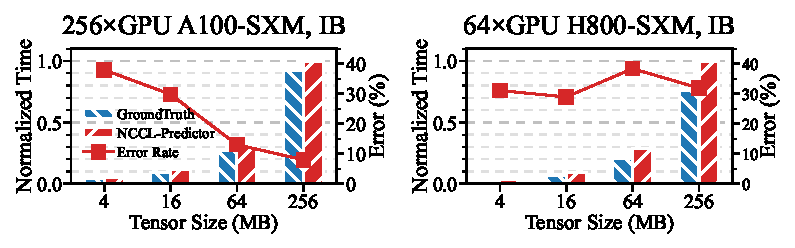
\includegraphics[width=1\linewidth]{figures/motivation/new_motivation_nccl_compare.pdf} 
    \vspace{-5mm}
    \caption{Comparison of predicted communication time (by NCCL-Predictor) and ground truth for \ar.}
    \label{fig:bw_compare} 
    \vspace{-3mm}
\end{figure}

The second, more precise approach involves white-box modeling specifically targeting collective communication (CC) \cite{won2023astra,SimAI2025NSDI}.
Since \nccl (and other CCLs too) implements a CC \op as an orchestrated series of P2P send and receive operations, we can simulate each send and receive to compose the end-to-end result. 
Similar to the training workloads, this naturally reflects the complex optimizations used by CCLs according to topology, NCCL P2P protocol (LL, LL128 or Simple), network interconnect (IB or RoCE), algorithm (ring or tree), etc.
To faithfully simulate the send/receive time, prior work \cite{won2023astra,SimAI2025NSDI} uses packet-level discrete-event network simulators like ns-3 \cite{riley2010ns}, which takes the physical topology and profiled link bandwidth as input.
Yet packet-level simulation is computationally expensive as it needs to simulate the entire protocol stack at each node in the network: 
We run the most recent SimAI \cite{SimAI2025NSDI} with an optimized multi-threaded ns-3, and observe that simulating a single iteration on a 128-GPU cluster takes over 2 hours (7655s) on a 32-core server.
% \fx{
% Extrapolating from this measurement, we find a direct design-space exploration for an 8{,}192-GPU system over 100 training configurations would require on the order of 1.5 years of simulation time (\cref{subsec:overall_perf}).
% In practice, this limits such simulator to a small number of high-fidelity case studies and makes them unsuitable for broad configuration sweeps or rapid training-strategy search (which is a basic ablity requirement for simluators).
% Therefore, the challenge is how to scale white-box communication simulation efficiently—preserving much of the accuracy of these detailed models while avoiding the prohibitive cost of packet-level simulation.
% }
\fx{
Extrapolating from this measurement, a direct design-space exploration for an 8{,}192-GPU system over 100 training configurations would require on the order of 1.5 years of simulation time (\cref{subsec:overall_perf}), effectively confining such packet-level simulators to a small number of high-fidelity case studies and making them unsuitable for systematic configuration sweeps or rapid training-strategy search. 
Thus, our second challenge is how to scale white-box communication simulation efficiently so as to retain much of the accuracy of these detailed models while avoiding the prohibitive cost of packet-level simulation.
}

% \fx{for a 8192 GPUs system design-space exploration over 100 training configurations (cref{}) the time will be 1.5 years. making such approach more suitable for a small number of high-fidelity studies rather than broad configuration sweeps, 非常限制了simulator的功能性。}
% Therefore, the challenge is how to scale the white-box communication simulation efficiently without sacrificing accuracy.


% We denote the slowdown factor to be the ratio between running time profiled with overlapping \ar kernel and the one without \ar kernel.
\vspace{0.3em}
\noindent \textbf{Challenge 3:}
\textit{How to account for the interference between overlapping computation and communication?}


\begin{table}[t]
    \scriptsize
    \centering 
    \resizebox{1\columnwidth}{!}{ 
        \begin{tabular}{@{}lll|ll@{}}
        \toprule
        Model       & Overlapped op & Slowdown & Kernel Type & Slowdown \\ \midrule
        VGG19       & 57.53\% & 37.67\%    & GEMM   & 26.95\%    \\
        GPT2        & 51.75\% & 10.61\%    & Sum    & 50.83\%    \\
        Llama3-8B   & 26.79\% & 7.15\%  & GroupedGEMM  & 11.78\%    \\
        Mixtral-8x7B  & 23.02\%  & 10.55\% & Grad   & 61.37\%    \\ \bottomrule
        \end{tabular}} 
    \caption{Statistics about (1) the proportion of overlapped kernels in different models and the slowdown factors in a training step, and (2) slowdown factors of some common computation \ops. Evaluated with PyTorch (VGG19), DeepSpeed (GPT2), Megatron-LM (Llama3-8B), and Flux~\cite{fluxgithub} (Mixtral-8$\times$7B).
    } 
    \label{table:model_kernel_slowdown} 
    \vspace{-4mm}
\end{table}

Overlapping computation and communication is widely used to improve efficiency and utilization~\cite{jiang2024megascale,chen2024centauri,zhang2017poseidon}.
We find that overlapping introduces non-negligible slowdowns especially to computation \ops, even though they are assigned to separate streams on the GPU.
Here, we define slowdown as the percentage increase in running time when overlapping communication kernels compared to no overlap.\footnote{
{Experiments here are conducted on the NVIDIA A800 cluster described in \cref{subsec:setup}, with software environment aligned to the configuration in~\cref{sec:implementation}.}
}
{
As shown in Table~\ref{table:model_kernel_slowdown}, at least 23\% computation \ops overlap with communication (across training frameworks), leading to a slowdown of up to 1.37x.
}
% Note here \ar as the communication operator overlapping with computation.
We also examine the slowdown to individual kernels.
Table~\ref{table:model_kernel_slowdown} (second column group) shows when overlapped with communication kernels with 25MB messages, running times of common kernels increase by an average of 37.73\%.
The CDF of slowdown factors for all computation kernels of Mixtral-8x7B is presented in Figure~\ref{fig:slowdown_cdf}, where slowdown can reach 800\% with an average of 79.2\%. 
Some recent work~\cite{hwang2023ark} also reported similar slowdowns in production training clusters. 
Despite its salient impact, overlap-induced slowdown has been overlooked by most existing work.
Proteus~\cite{duan2024proteus} uses a simple heuristic factor that varies only with GPU architecture and ML model to account for this slowdown, which is too coarse to be accurate and not generalizable to unseen models.

Simulating the overlap-induced slowdown is a daunting task. 
Ideally, we need to model the kernel-level behavior in order to know exactly how the kernels overlap.
For example, in the widely-used gradient overlap optimization~\cite{zhang2017poseidon}, the simulator must correctly replay the backpropagation computation kernels and schedule communication kernels at precise times to achieve accurate overlap.
Further, for a given computation kernel, its slowdown factor is influenced by various factors of hardware and software setup. 
Table~\ref{table:slowdown_env} shows the slowdown factors of two kernels on different GPUs and CUDA versions vary a lot.
This is because the kernel implementation and resource scheduling ultimately determines how GPU resources are shared and contended among concurrent kernels.
These proprietary details are inaccessible for us, not to mention the complexity of modeling them.
% Thus, how to practically simulate the effect of overlapping computation and communication remains a formidable challenge.


\begin{figure}[t]
    \begin{minipage}{0.26\textwidth}
        \centering 
        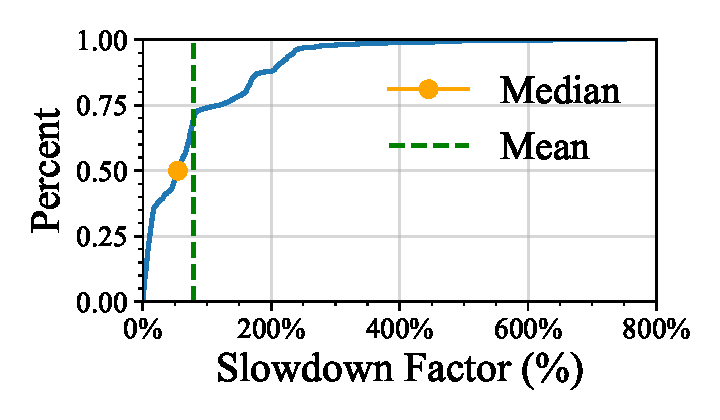
\includegraphics[width=\linewidth]{figures/motivation/slowdown_cdf_positive.pdf} 
        \caption{{CDF of slowdown factor of kernels in Mixtra-8x7B.}} \label{fig:slowdown_cdf} 
    \end{minipage}%
    \hfill
    \begin{minipage}{0.2\textwidth}
        \centering
        \small
        \resizebox{\linewidth}{!}{
            \begin{tabular}{@{}llcccc@{}}
            \toprule
            GPU & Kernel        & CUDA & Slowdown \\ \midrule
            \multirow{4}{*}{\centering 3090}         & GEMM       & 11.8  & 26.4\%     \\
                                                     & GEMM       & 12.1  & 39.3\%      \\
                                                     & LayerNorm  & 11.8  & 18.0\% \\
                                                     & LayerNorm  & 12.1  & 93.8\% \\ \midrule
            \multirow{4}{*}{\centering A800}         & GEMM       & 11.8  & 13.4\% \\
                                                     & GEMM       & 12.1  & 17.8\% \\
                                                     & LayerNorm  & 11.8  & 9.1\% \\
                                                     & LayerNorm  & 12.1  & 20.7\% \\ \bottomrule
            \end{tabular}}
        \captionof{table}{Slowdown of some kernels across GPU architectures and CUDA versions.}
        \label{table:slowdown_env}
    \end{minipage}
    \vspace{-5mm}
\end{figure}


%!TEX root = main.tex 


\section{Design Overview} 
\label{sec:overview} 

\noindent Building upon the aforementioned observations and motivations, 
we introduce \sys, a simulator tailored for large-scale LLM training.

\begin{comment}
\vspace{0.2em}
\noindent\textbf{Design objective.}
A performance simulator should predict the step time of a training model with minimal effort while providing high-quality runtime statistics for each stage of the training process. Our primary objective is to design an accurate simulator that reduces the need for repetitive and costly experiments. We focus on large-scale distributed training for two key reasons: (1) Large-scale training is particularly expensive, and we expect that \sys can significantly reduce costs. (2) Large-scale distributed training often experiences greater performance degradation due to device communication, making it more challenging to identify bottlenecks and optimize efficiency.
\end{comment}

\noindent\textbf{Key design choices.}
% \hxq{highlight and explain the key design choices of \sys.}
We highlight the key choices in building \sys to address the three challenges in \cref{subsec:challenges}. 
% previous methods for extracting training workloads typically involve either running on physical clusters (trace-based approaches) or incurring significant manual labor (manual-based approaches). 
\begin{itemize}[leftmargin=*]

\item To obtain training workloads without a full-scale deployment, \sys employs a novel ex-situ tracing approach. 
Generally, ML frameworks support various parallelism in the following way: (1) they initialize each rank (typically one rank per device) with its own sub-model based on the parallelism setting, and then (2) each rank builds its own execution graph to start actual training. 
\sys turns this parallel process into a sequential one, using only one device to act as each rank iteratively to trace the corresponding execution graph and profile the running time of each \op at the same time, achieving faithful workload tracing without requiring the full cluster.

% \sys strikes a balance between these extremes by developing a generalized tracer, compatible with mainstream training frameworks such as DeepSpeed, and Megatron-LM. While our approach (\cref{sec:workload_const_replay}) remains trace-driven to ensure the precision of \wg{}s, it eliminates the resource constraints of traditional methods, allowing users to capture distributed training workloads from a single standard GPU, significantly reducing the cost of workload extraction.

\item To achieve accurate and efficient communication simulation, \sys employs a white-box modeling approach with empirically profiled parameters that strikes a good balance between accuracy and efficiency.
% This compromise involves constructing a generalized formulation of the communication process 
Our model is derived closely after NCCL's underlying chunk-based implementation of collective communication capturing critical factors such as per-chunk inter-server transmission time. 
These factors are profiled offline exhaustively to capture the complex dynamic optimization by \nccl according to hardware features and software configurations.

\item To account for the interference between overlapping computation and communication, \sys adopts a black-box method using features related to both computation and communication kernels, such as bucket size, SM occupancy, and cache hit rate.
\end{itemize}
% The model is trained using kernel performance data from single-device runs and the parameters of communication setting to predict their interaction and resulting slowdown.
% \hxq{merge this with the overall arch}
% \noindent\textbf{System input.}
% \sys requires three inputs: (1) User variable: This describe the selected training framework (e.g., PyTorch, DeepSpeed, Megatron-LM), training strategy details (e.g., 3D parallelism, overlap), and simulation settings such as profiling scope and iteration count. (2) Model configuration: This includes model settings such as structure, hyperparameters (e.g., hidden size, number of layers, bucket size). (3) Hardware configuration: This specifies the physical cluster setup, including cluster size, network topology (both intra- and inter-server), and NCCL environment parameters (e.g. NCCL\_TOPO\_FILE, NCCL\_BUFFSIZE).


% \vspace{0.2em}
% \noindent\textbf{System architecture.} 
% Figure~\ref{fig:arch} illustrates the architecture of \sys.
% The \textit{\extractor} constructs the training workload using tailored modules for tracing \wg. 
% It generates detailed workload information, including computation and meta-information for communication workloads, using an enhanced tracing approach, and performs quick GPU memory checks to validate the training plan (i.e., out-off-memory check). The \textit{\cm} predicts the runtime of communication kernels (\cref{sec:comm_pred}). It includes a network performance benchmarking module optimized for NCCL, capable of formulating communication functions based on the profiled dataset. The \textit{\ma} replays the training process (\cref{subsec:workload_replay}). It reorganizes the execution sub-graphs of all GPUs and schedules the operators in global timelines, accurately simulating the training behavior. The \textit{\va} adjusts the runtime of overlapped kernels based on a ML approach to reflect slowdown inferences (\cref{sec:overlap_pred}). Additionally, \sys embeds a \textit{database} to store and share profiling data, facilitating predictions and reducing redundant profiling.

% \fx{hx:merge this with the overall arch}
\noindent\textbf{System architecture.}
Figure~\ref{fig:arch} shows \sys's architecture.
Its input includes three categories: user-defined settings specifying the training framework, parallelism strategies (DP/TP/PP/EP groups); model details defining the model structure and hyperparameters; and hardware configurations detailing device specifics (GPU type), cluster size, network topology, \nccl parameters (e.g., NCCL\_TOPO\_FILE, NCCL\_BUFFSIZE), etc.
Given these inputs, the \textit{\extractor} extracts training workloads for each rank, including the per-rank execution graph and \op running times (\cref{subsec:workload_const}). 
% It employs an enhanced tracing approach to generate detailed computation and communication workloads, and performs quick memory checks to detect insufficient memory conditions, reporting out-of-memory errors when necessary.
The \textit{\cm} module (\cref{sec:comm_pred}) leverages the white-box models with parameters corresponding to the given settings to estimate each communication kernel's performance. 
Then the \textit{\ma} module (\cref{subsec:workload_replay}) re-constructs the global timelines of the end-to-end training process by assembling all per-rank execution graphs with estimated communication \op performance and inter-rank dependencies. 
The \textit{\va} module (\cref{sec:overlap_pred}) applies a machine learning model to adjust the running times of overlapping operations, accounting for the interference-induced slowdown, and outputs the final training step time result.  
Additionally, \sys maintains a \textit{database} for profiling data, reducing redundant measurements across simulations.

% \noindent\textbf{System workflow.} 
% \sys begins by analyzing the provided inputs.
% The \textit{\extractor} then loads the model on a single GPU to derive execution sub-graphs for all devices involved iteratively. If a requested operation's profile is not already in the database, \sys profiles it and stores the result. For communication operations, the \textit{\cm} uses the profiled data based on a white-box approach to predict their runtimes. Once all sub-graphs are collected, the \textit{\ma} arranges them in global timelines. When operations overlap, the \textit{\va} adjusts their runtimes to reflect realistic slowdowns. Finally, \sys produces a comprehensive performance report.


\begin{figure}[t] 
    \centering 
    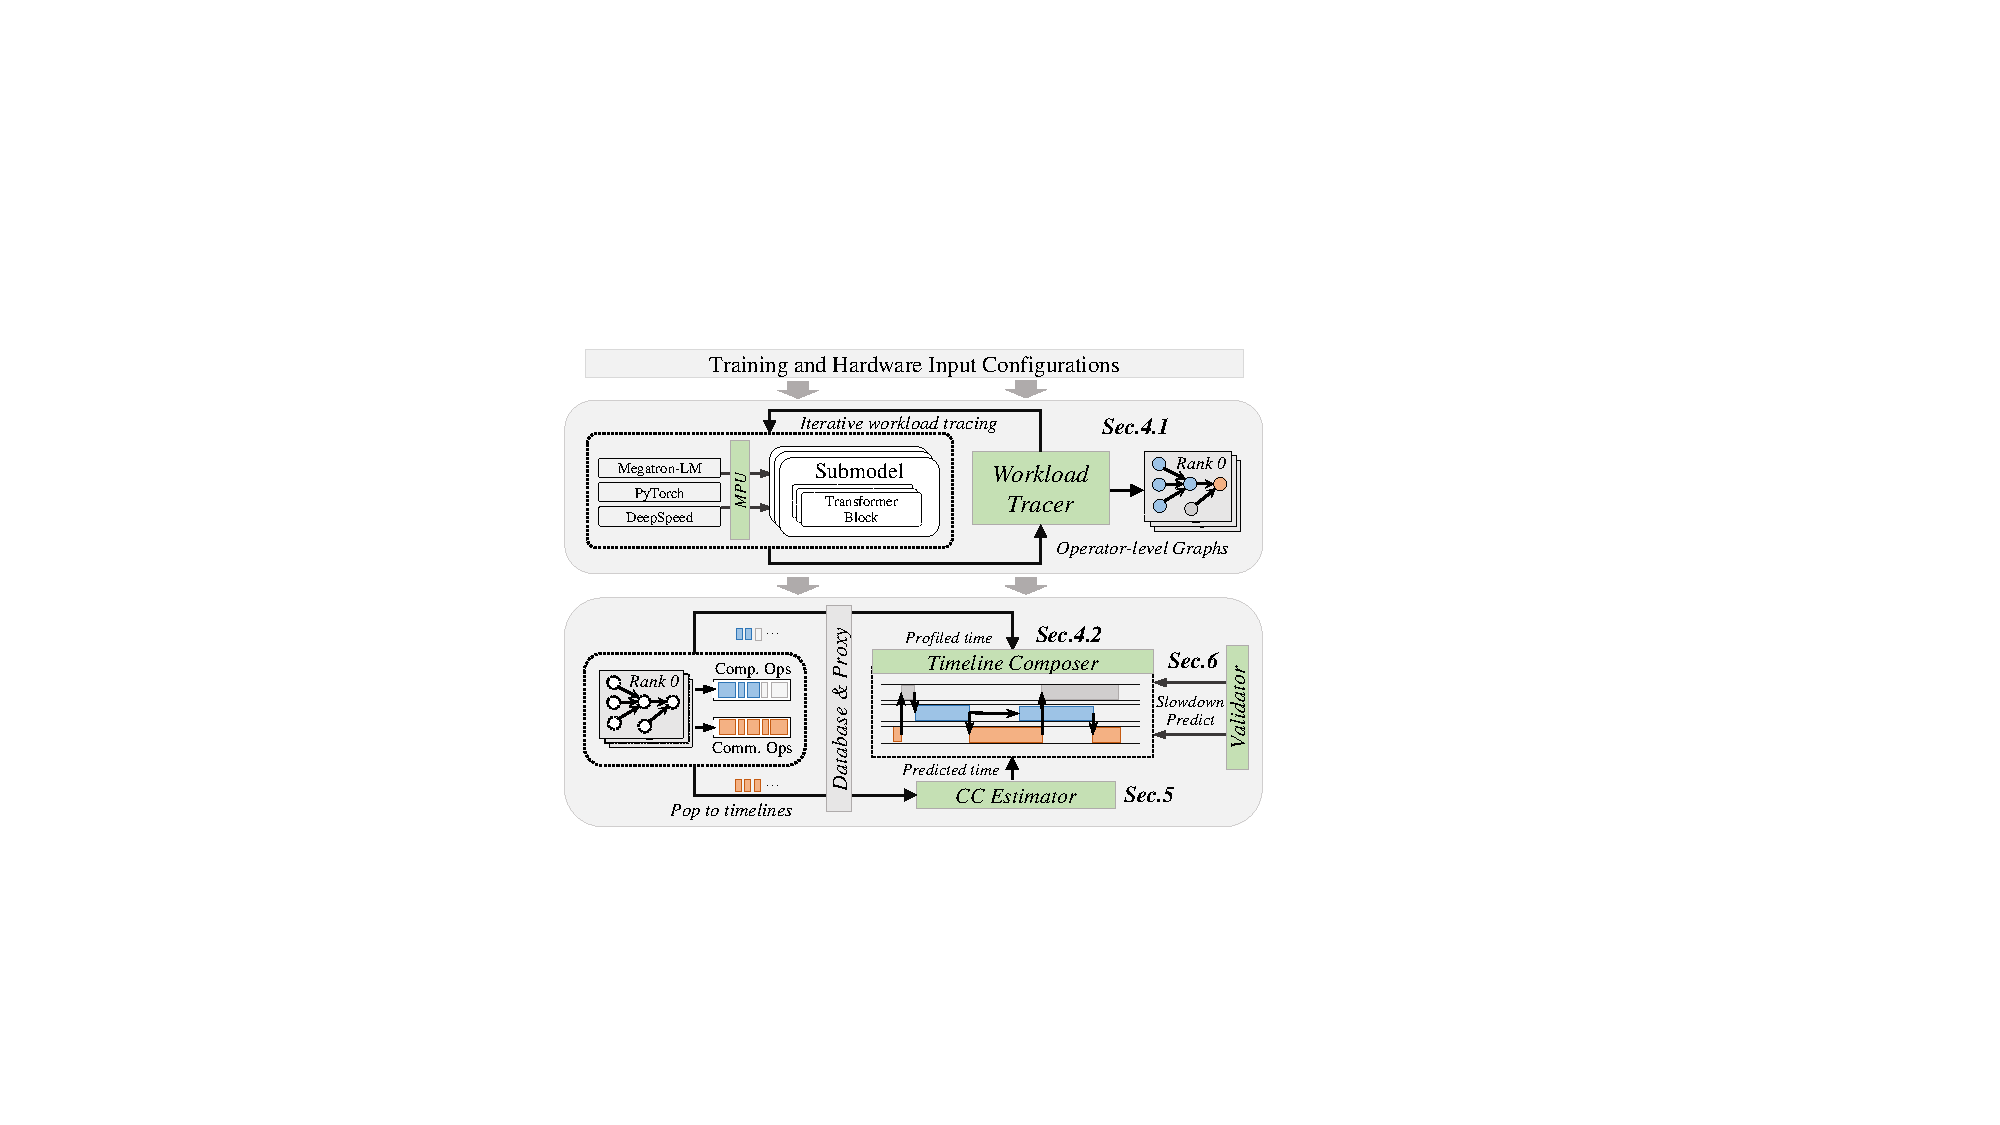
\includegraphics[width=\linewidth]{figures/design/moye_overview.pdf} 
    \caption{\sys architecture overview. The green components represent the core modules of \sys.} 
    \label{fig:arch} 
    \vspace{-1.5em}
\end{figure}



% In \sys, we center around two key questions: 
% \begin{itemize}[leftmargin=3mm] 
%     \item How to accurately estimate the all-reduce running time given a large-scale cluster configuration? 
%     \item How to predict the slowdown factor of kernels that are interfered by the concurrent all-reduce kernel? 
% \end{itemize}


%!TEX root = main.tex 

\section{Workload Tracing } 
\label{sec:workload_const_replay} 

% We first present in this section how \sys accurately traces the training workloads for each rank in an ex-situ fashion using a single device, thereby addressing Challenge 1 (\cref{subsec:challenges}). 
% We also show how \sys composes the global timelines across devices using the per-rank workloads to faithfully re-construct the entire training process in \cref{subsec:workload_replay}.



% 1. per-rank workload tracing;
% 2. replay to recover global timelines

\subsection{Per-Rank Workload Tracing} 
\label{subsec:workload_const}

% Generally, ML frameworks support various parallelism in distributed training in the following way: (1) they initialize each rank (typically one rank per device) with its own sub-model based on the parallelism setting, and then (2) each rank builds its own execution graph to start actual training. 
% As discussed in \cref{sec:overview}, \sys turns the parallel initialization process into a sequential one during job deployment to achieve faithful workload tracing without requiring the full cluster.
% \noindent \textbf{Iterative submodel initialization.}

To launch a training job, the ML framework registers the global parallelism parameters (e.g. DP/TP/PP/EP groups) given by user into the so-called model parallelism unit (MPU), which maintains all states related to parallelisms for a given rank.
Then according to the MPU, each rank concurrently initializes its own part of the model that it needs to train for (Figure \ref{fig:profier} \textcircled{1}
), and starts training with an execution graph that is optimized for its submodel based on the hardware/software environment and user configurations. 

\sys extracts the per-rank execution graph in an ex-situ fashion by transforming the above parallel process into a sequential one (Figure \ref{fig:profier} \textcircled{2}
). 
Specifically, \sys hijacks all the calls to the original MPU and re-directs them to its own MPU, and registers the global parallelism parameters as usual.
\sys's MPU only manipulates the input arguments to the MPU when necessary; it does not change the original implementation to ensure correctness.
Then with a single device, in each iteration $i$, \sys uses this unique rank ID $i$ to initialize the corresponding submodel and execute one complete training step, so all information regarding the computation \ops, including their dependencies (including those w.r.t other ranks) and running times, can be profiled.
For MoE workloads, \sys provides an interface to control token distributions across experts.
To ensure execution isolation, \sys launches each simulated rank as a separate single-process \texttt{torchrun} job, mirroring real distributed execution. Thus, the GPU only needs to hold one rank's model shard and step-local states at a time, so the memory requirement follows the largest per-rank shard under the target parallel configuration rather than the aggregate memory of all ranks.
Within this isolated execution, \sys runs the actual compute path for the current rank and samples GPU memory online, capturing allocator-level dynamics such as activation allocation, reuse, and early deallocation. Our current validation therefore focuses on per-rank training-step memory behavior excluding communication-time execution (see~\cref{subsec:workload_perf}).


The caveat here is collective communication: one device obviously cannot execute a communication \op. 
To resolve this, notice that when the communication \op is launched it also needs to call into the MPU which determines the device's position in the global communication groups for proper execution.
This is re-directed to \sys's MPU again allowing it to trace the communication \op's truthful information in the simulated setting (group association, message sizes, etc.); meanwhile, instead of returning results using the simulated (distributed) setting, \sys's MPU returns results corresponding to single device setting, so the communication \op can proceed and training is not blocked. 
This way \sys traces the actual execution graphs for each rank and running times of computation \ops without requiring the full-scale cluster.
Implementation details of tracing vary across frameworks which we will discuss in \cref{sec:implementation}.

\begin{figure}[t] 
    \centering 
    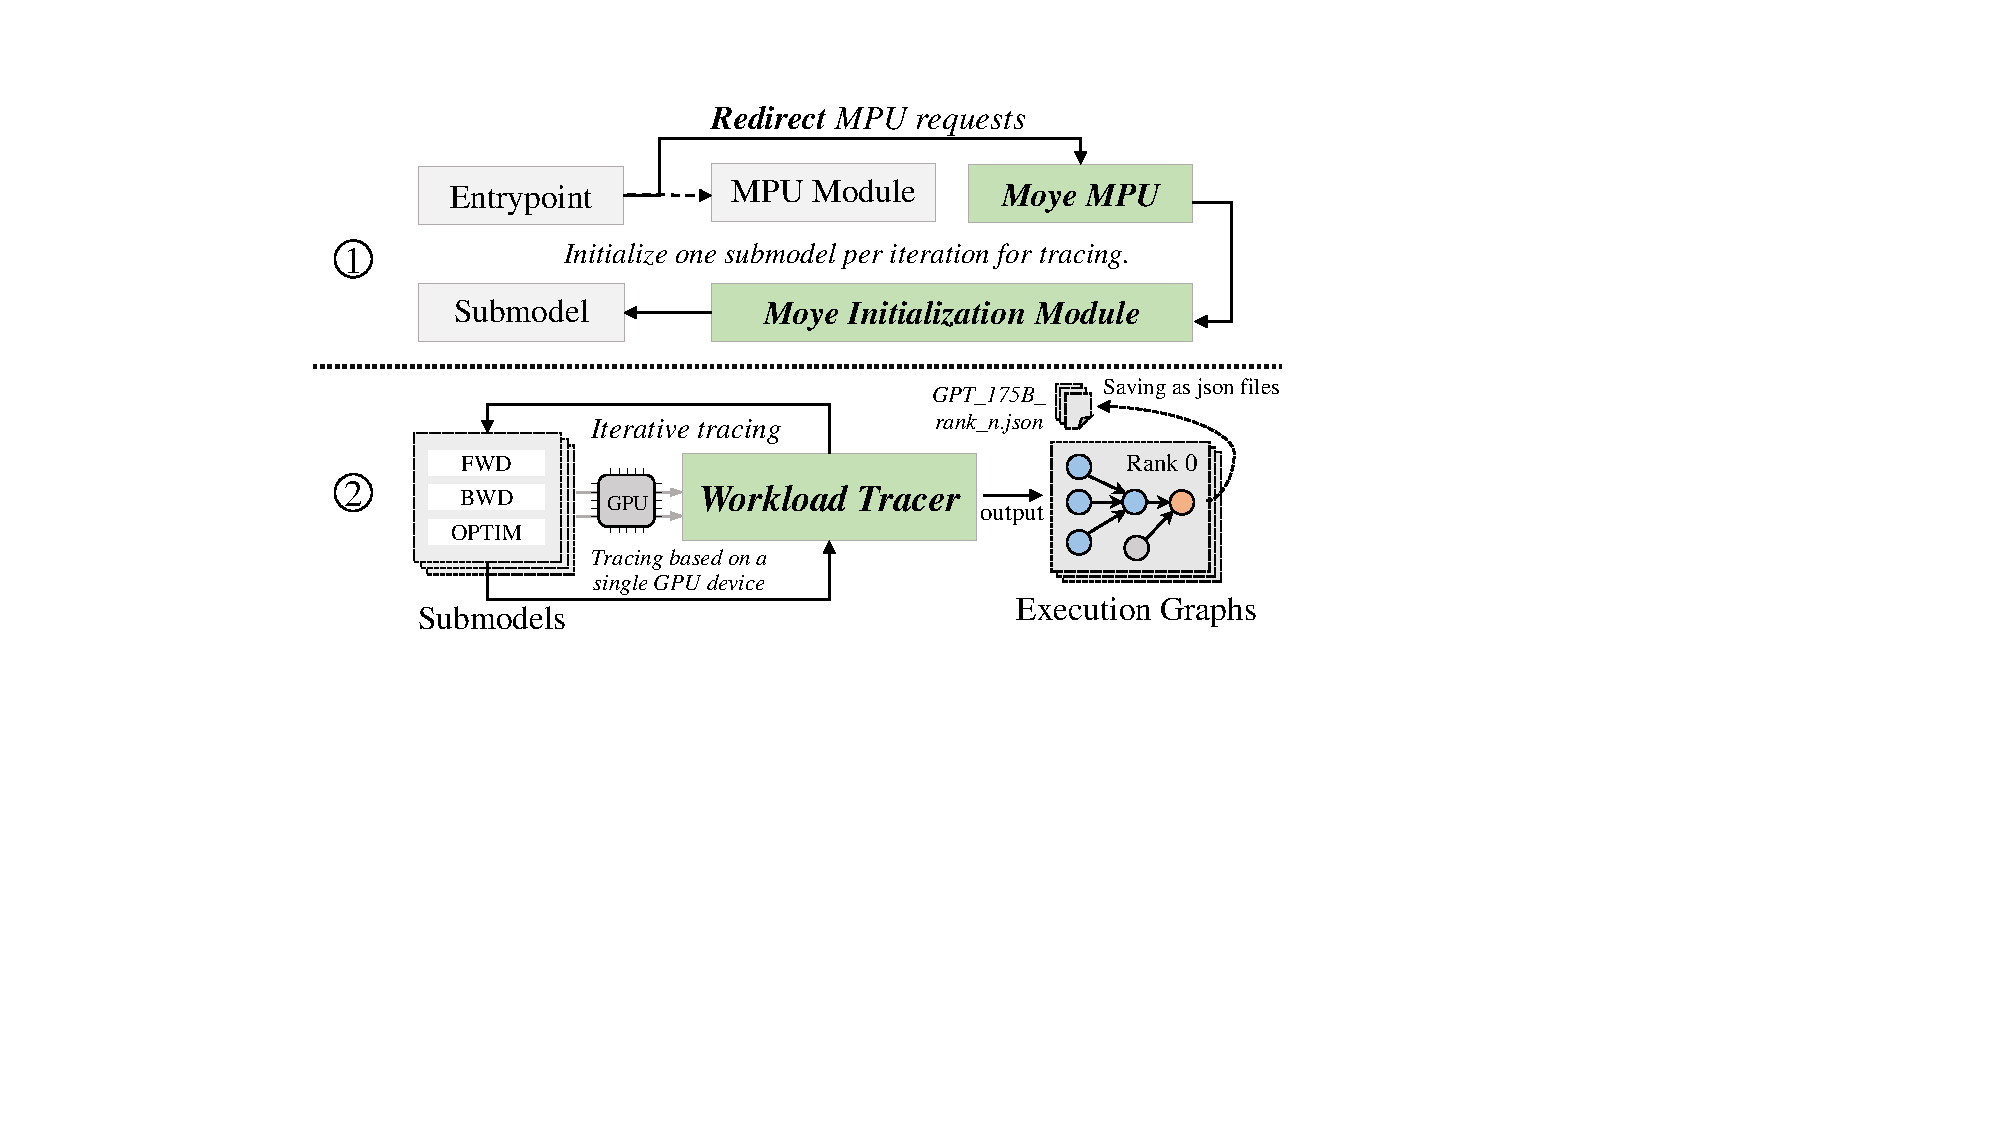
\includegraphics[width=\linewidth]{figures/design/moye_workload_tracer.pdf} 
    % \vspace{-2em}
    \caption{\sys's MPU module and workload tracer.} 
    \label{fig:profier} 
    \vspace{-1em}
\end{figure}

Note that after per-rank workload tracing, all collective communication \ops on the per-node execution graph are placeholders without any running time.
The job of \sys's \cm and \va is precisely to estimate and refine the communication times, respectively, in the next phase.
% In 3D parallelism, generating the complete workload for a training job involves three key steps. First, the model parameters are parsed (e.g., model structure, parallel training settings). Then, the model parallel unit (MPU) module uses these parameters to determine the submodel structure for each rank (typically, one rank per GPU). Finally, each rank initializes its submodel, moving it to the appropriate GPU. \sys allows users to pass simulation-specific parameters to initialize a simulated training environment within the current training framework. 

% When the simulation environment is activated, calls to the standard MPU are redirected to \sys's MPU module, which replaces the original parameters with simulated ones (e.g., number of GPUs, PP and TP configurations). As a result, \sys can determine the submodel to be deployed on each rank. However, at this point, \sys cannot directly execute forward or backward passes on these submodels, as their module implementations contain communication operations (e.g., all-reduce in TP). By restricting the visible GPUs to a single device through \sys's MPU module, \sys bypasses communication dependencies, enabling accurate execution of the workload on a single GPU. To ensure all ranks' workloads are properly initialized, \sys performs this initialization iteratively, simulating distributed behavior without requiring physical cluster resources.

% Unlike previous tools, which often segment the graph when encountering communication operators, \sys treats communication operations as placeholders within the \wg, recording their meta-information (e.g., group associations, message sizes, etc.) and positions within the graph. These placeholders are later replaced with actual runtime estimates during the communication simulation phase~(§X) \jz{(fix this)}. Additionally, \sys provides a lightweight context manager that allows users to adjust the granularity and scope of the trace. For instance, in Megatron-LM's 3D parallelism mode, \sys allows multiple computation operations to be merged into a single operation for simplification. 





\subsection{Timeline Composing } 
\label{subsec:workload_replay}
% \jz{(Workload replay is performed after communication estimator. So this part should be moved to the back?)}

\noindent Before presenting the communication estimation and validation, we discuss how \sys obtains the end-to-end training step time by composing the global timeline with the per-rank workloads obtained above.
%  \ma simulates the end-to-end training process by replaying the per-rank execution graphs.  

Assuming all communication running times are known, \sys's \ma can recover the training process by replaying the per-rank execution graphs.
%  according to the dependencies encoded within. 
\ma is an event-driven simulator that walks through the per-rank execution graphs and puts all \ops (events) onto the global timelines accordingly, including the computation timeline, communication timeline, and memory copy (memcpy) timeline. 
As shown in Figure~\ref{fig:timeline}, a critical piece of information missing from the per-rank graphs is dependencies across ranks; for instance the downstream stages in rank $i$ requires activations from the upstream stages in rank $i-1$ before starting the forward computation in PP.
We provide predefined dependencies and matching rules for both inter-stage and intra-stage events for common parallelism strategies, such as 1F1B.
To enhance flexibility, this module is exposed as an API, allowing users to input new dependencies and matching rules for custom strategies.

While it is possible to strictly replay dependencies through every synchronization across all communication groups, this would significantly increase the timeline construction overhead. 
Instead, \sys leverages workload characteristics to selectively relax synchronization in order to accelerate simulation. 
For instance, in dense models, since each TP rank processes identical sequence lengths, the computation is inherently balanced, allowing us to ignore synchronization delays in TP all-reduce. 
For MoE models, however, load imbalance in the FFN layers requires \sys to preserve the full dependency logic to ensure correctness. In MoE workloads, this conservative treatment is necessary because expert dispatch, expert compute, and expert combine are no longer uniform across ranks: routing imbalance can make a subset of EP ranks the critical-path stragglers. Relaxing these dependencies would therefore bias both tail latency and end-to-end step time.

% Events are mapped to the corresponding timeline based on their attributes.


\begin{figure}[t] 
    \centering 
    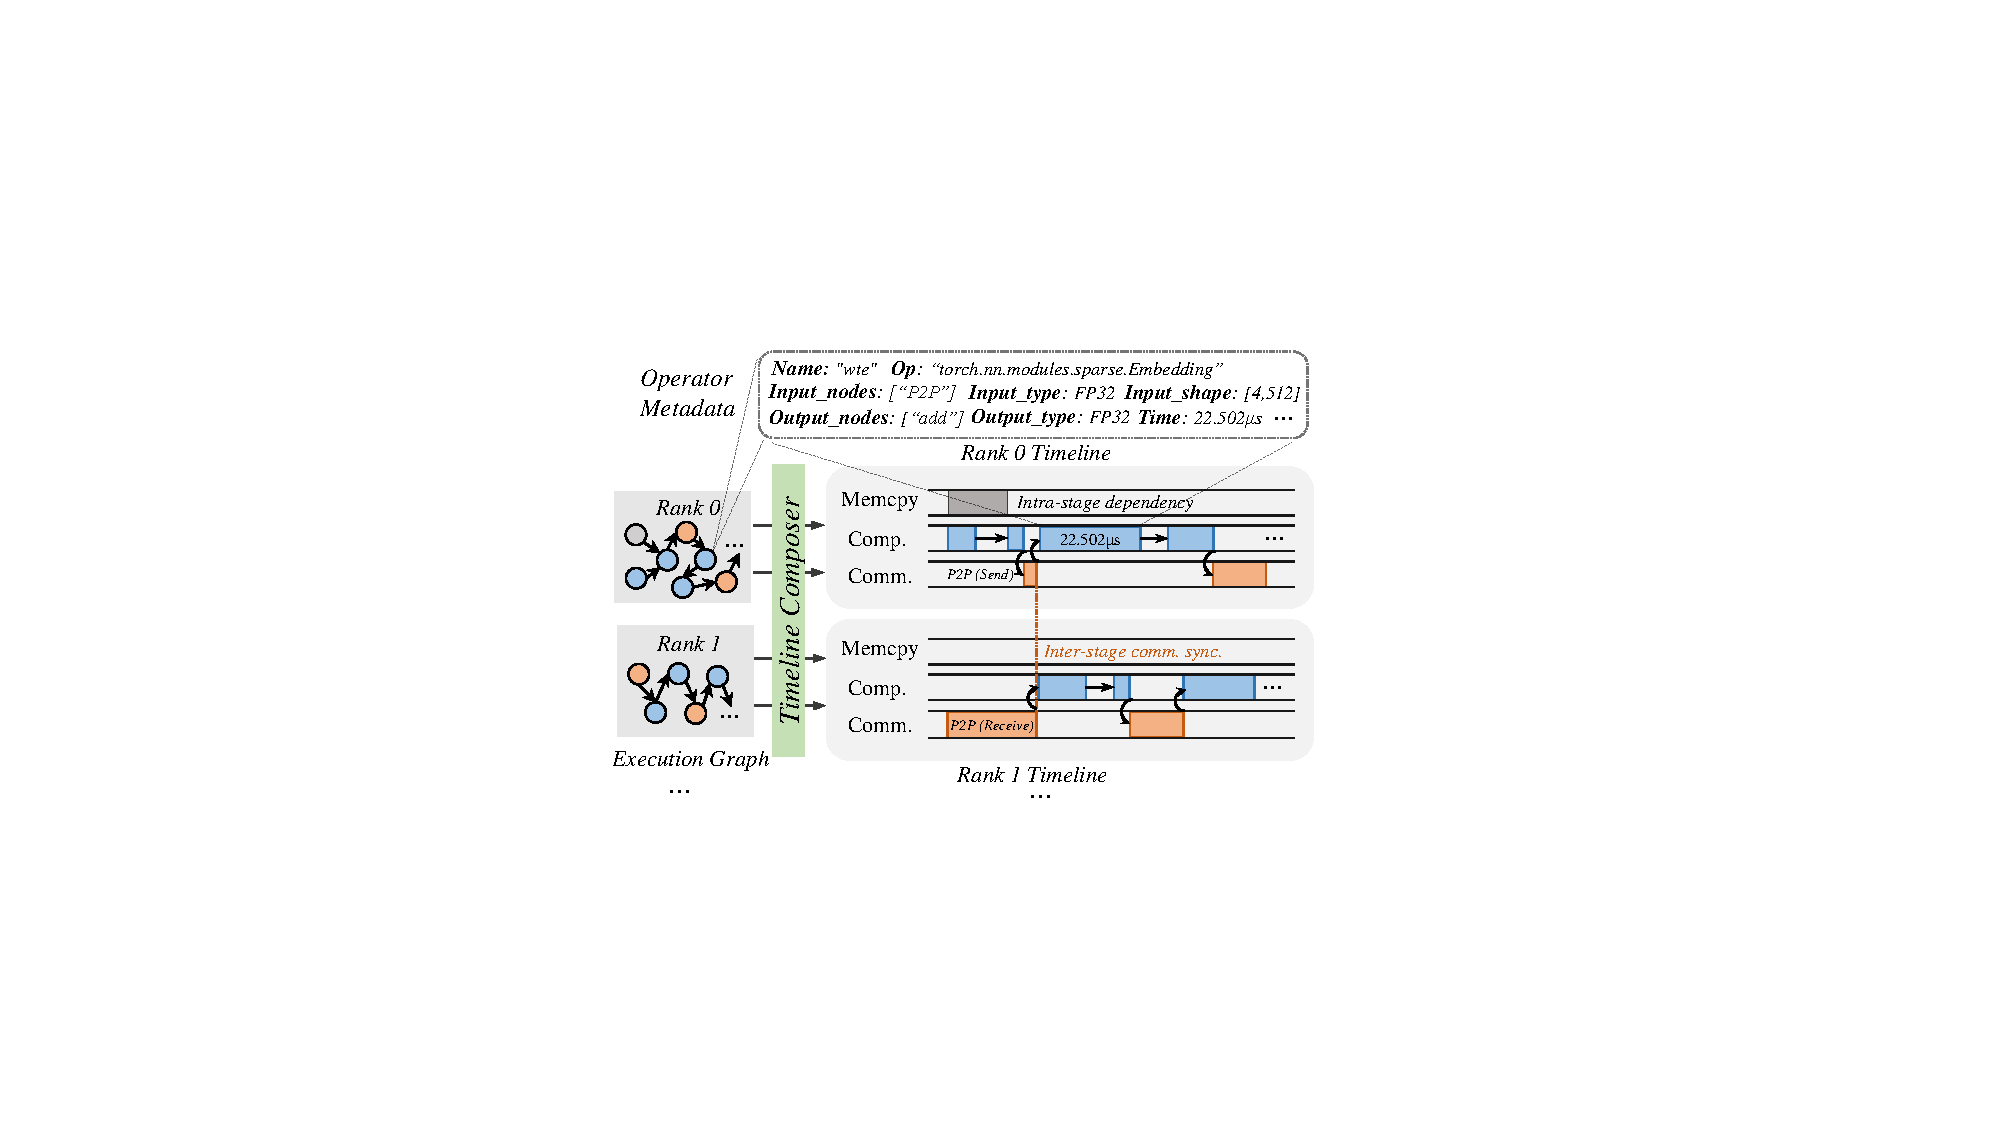
\includegraphics[width=\linewidth]{figures/design/moye_timeline.pdf} 
    \vspace{-1.5em}
    \caption{Illustration of how \sys schedules operations in the execution graph to timelines across ranks.} 
    \label{fig:timeline} 
    \vspace{-1em}
\end{figure}

% \noindent \textbf{Dependencies managing.}
% Additionally, \sys includes predefined dependencies and matching rules for both inter-stage and intra-stage events. For example, in a 1F1B scheduling strategy, downstream stages wait for activation data from upstream stages before starting forward computation. 

\section{Communication Modeling}
\label{sec:comm_pred}

\subsection{Background on \nccl} 
\label{subsec:tree_allreduce}
\nccl provides collective communication (CC) functions as single CUDA kernels \cite{nccl} to support various training parallelisms. Our models therefore predict performance at the kernel level, a close approximation that ignores negligible launch overheads (the same applies to the slowdown prediction in \cref{sec:overlap_pred}). 
A key \nccl feature is pipelining messages as smaller equal-sized chunks, which is the basis for our formulation in \cref{subsec:whitebox_modeling}. For its \ar collective, \nccl supports both ring-based \cite{nccl} and tree-based \cite{tree} algorithms. Other CC kernels use ring-based algorithm only.

\subsection{White-Box Modeling: Synchronization}
\label{subsec:whitebox_modeling}

\noindent \sys models a \nccl kernel as two sequential stages: synchronization and execution. Upon invocation, the kernel first checks whether it can start execution based on the readiness of ranks in the current communication group. If not all ranks are ready, the kernel waits for synchronization before it can proceed. 
Thus, the total running time of a kernel is the sum of synchronization time and execution time.
Here we investigate the synchronization time first. 

\sys models synchronization time after \nccl's implementation logic.
%  which varies across communication kernels, as illustrated in Figure~\ref{fig:comm_sync_logic}.
For P2P \send and \recv, it waits until its target communicator (i.e., each rank's communicator instance) is ready to proceed. 
In contrast, for CC kernels, the communicator associated with each rank in the current group must wait until all communicators have been successfully launched. 
The last communicator to initiate determines the actual start time of this kernel.
\sys's synchronization model captures the impact of stragglers by simulating their effect on communication delays.


% 请确保在您的文档导言区（preamble）包含了 \usepackage{booktabs}
\begin{table}[t]
\centering
\small
\renewcommand{\arraystretch}{0.8}
\begin{tabular}{cccc}
\toprule
\#GPUs & conn\_setup & data\_reduction & total\_trans \\
\midrule
32  & 7.3\% & 31.7\% & 61.0\% \\
64  & 6.4\% & 38.3\% & 55.3\% \\
128 & 5.8\% & 46.2\% & 48.1\% \\
256 & 5.4\% & 39.3\% & 55.4\% \\
\bottomrule
\end{tabular}
\caption{\fx{Breakdown of running time of \nccl \ar kernel (as percentage of total time) with varying GPU counts, profiled on standard A100-SXM IB-connected clusters. The total\_trans includes both intra- and inter-trans time.}}
\label{table:runtime_percentage}
\vspace{-2em}
\end{table}



\subsection{White-Box Modeling: Execution}
\label{subsec:whitebox_modeling}


\noindent Execution time represents the majority of kernel running time, and is the focus of our modeling. We build white-box models that closely follow the kernel execution process in \nccl under different algorithms, and profile all key parameters of the models exhaustively in various hardware/software settings to achieve accurate prediction without the high overheads of event-based simulation.

\noindent\textbf{Basic model.}
\fx{We perform a running time breakdown analysis of CC kernel in Table~\ref{table:runtime_percentage}.
By inspecting \nccl's GPU-side implementation~\cite{nccl-implement, hu2025demystifying} and tracing the control flow of CC kernels}, we find that the execution time of a CC kernel can be decomposed into (at most) four \textit{non-overlapping} phases, using \ar as an example:
\begin{equation} 
    \begin{split} 
        T_{comm\_kernel} = & T_{conn\_setup} +T_{intra\_trans} 
        \\ & +T_{data\_reduction} +T_{inter\_trans}
    \end{split} 
    \label{eqn:cc_basic} 
\end{equation}
Here $T_{\text{conn\_setup}}$ is connection setup time; $T_{\text{intra\_trans}}$, $T_{\text{inter\_trans}}$ are the times to transmit tensor chunks according to the specific algorithm, and $T_{\text{data\_reduction}}$ is the computation time of the reduce operation over the received tensor chunks and the local tensor. 
Note that not all four components are present in other CC kernels. 
\fx{Thus, this decomposition is implementation-faithful rather than an empirical regression artifact.}

Building on Eq.~(\ref{eqn:cc_basic}) \fx{and following the per-round send/recv schedule encoded in \nccl's ring and tree kernels~\cite{nccl-implement, nccl-ring-tree, hu2025demystifying}, we derive the following execution-time models for common CC kernels:}
% Building on Eq.~(\ref{eqn:cc_basic}), we formulate the following execution-time models for common CC kernels and algorithms:
\begin{align}
    T^{Ring}_{all-gather} = &\ \alpha + \gamma\cdot \eta (N-1), \label{eqn:44}\\  
    T^{Ring}_{reduce-scatter} = &\ \alpha +  \eta\big[(N-1) + \gamma \times (N-1)\big]\nonumber\\
                            &  + \delta \times tensor\_size, \label{eqn:33}  \\
    T^{Ring}_{\ar} =&\ \alpha + \eta\big[(N-1) + \gamma \times 2(N-1)\big]\nonumber\\
                        &\ + \delta \times tensor\_size , \label{eqn:11} \\
    T^{Tree}_{\ar} =&\ \alpha + \gamma (\eta-1) +  2\beta(K-1) \nonumber\\
                    &\ + 2\gamma\log_2(M) + \delta \times tensor\_size. \label{eqn:22}
\end{align}
Here $N$ is the total number of devices, $M$ the number of nodes (servers), and $K = N/M$ the number of devices per node. We denote the connection setup time as $\alpha$, and the intra-server and inter-server transmission times as $\beta$ and $\gamma$. The reduce time depends on $\textit{tensor\_size}$ and the reduce throughput $\delta$. Finally, $\eta$ is the number of rounds (or chunks) for this tensor, which corresponds to \nccl's chunk-based implementation.

\yc{
Our white-box framework naturally extends to the \texttt{all-to-all} collective. 
Instead of using dedicated ring or tree algorithms, \nccl implements \texttt{all-to-all} by decomposing it into $N$ concurrent point-to-point \send and \recv pairs~\cite{nccl-implement}. 
These are executed by the \texttt{sendrecv} kernel using chunk-based pipelining. 
We model its execution time as:
\begin{equation}
    T^{P2P}_{\texttt{all-to-all}} = \alpha + \max\!\big(\beta \cdot \eta(K-1),\; \gamma \cdot \eta(N-K)\big),
\label{eqn:alltoall}
\end{equation}
where the $\max$ operator reflects the concurrent utilization of independent physical channels for intra-node (to $K-1$ GPUs) and inter-node (to $N-K$ GPUs) transfers. 
The $\delta$ term is absent since \texttt{all-to-all} involves no reduction. This collective is the key communication primitive for MoE expert dispatch and combine in our Qwen3-A3B and DeepSeek-V3-style workloads. Rather than approximating these exchanges with all-reduce-like behavior, \sys models them explicitly as chunked point-to-point transfers and combines this with its synchronization model to capture delays introduced by straggling ranks.
}

This modeling decouples scale-dependent terms from fabric-dependent parameters: job scale and parallelism enter only through $N, M, K, \textit{tensor\_size}$, and $\eta$, while $(\alpha,\beta,\gamma,\delta)$ summarize the steady-state behavior of intra- and inter-node communication for a fixed hardware/software stack. Once these parameters are calibrated on a moderate-size cluster, the same closed-form expressions can be evaluated for much larger $N$ and $M$ without additional network-level simulation.

% \noindent\textbf{Scale-dependent correction factor.}
The above models treat $\gamma$ as a per-hop inter-server transmission time that is primarily determined by the underlying hardware, software, and \nccl configuration. In practice, large jobs may incur additional latency from multi-tier topologies and aggregate flow-level contention that are not constant across scales. To capture these second-order effects without resorting to packet-level simulation, \sys introduces a dimensionless scale correction factor $c_{\mathrm{scale}}(N)$ and defines an effective inter-server transmission time
% \vspace{-0.25em}
\begin{equation}
\gamma_{\mathrm{eff}}(N)
  = \gamma \cdot c_{\mathrm{scale}}(N),
\label{eq:gamma_eff}
\end{equation}
% \vspace{-0.25em}
where $c_{\mathrm{scale}}(N) \geq 1$ aggregates residual scale-dependent network effects at job size $N$; its dependence on the \nccl algorithm and cluster topology is left implicit for brevity. During prediction, \sys evaluates equations by substituting $\gamma_{\mathrm{eff}}(N)$ for $\gamma$, so that the analytic dependence on $N$, $M$, and $K$ captures the dominant algorithmic scaling behavior, while $c_{\mathrm{scale}}(N)$ adjusts for large-scale contention.

\noindent\textbf{Offline exhaustive profiling.}
The modeling above is explicitly related to nine parameters and implicitly to an additional parameter, $\textit{chunk\_size}$. Among them, $N$, $M$, $K$, and $\textit{tensor\_size}$ are user configurations, while $\alpha$, $\beta$, $\gamma$, $\delta$, and $\eta$ are what \sys attempts to obtain. Modeling them analytically is challenging. First, they depend on $\textit{chunk\_size}$ and $\textit{tensor\_size}$. The chunk size is not a predefined constant but dynamically tuned by \nccl~\cite{nccl}. Further, these parameters vary with hardware configuration and software implementation (e.g., InfiniBand vs.\ NVLink, \nccl version). These idiosyncrasies also differ across CCLs, making a single closed-form model difficult.

We therefore adopt offline profiling to obtain these parameters, as they are fixed once the hardware/software configurations are settled. First, we modify \nccl to obtain the chunk size during the initialization phase. We enumerate representative combinations of $N$, $M$, $\textit{tensor\_size}$, and hardware type (InfiniBand, TCP, NVLink) to record the corresponding $\textit{chunk\_size}$ and number of rounds $\eta$ computed by \nccl. Then, for each $\textit{chunk\_size}$, we profile the corresponding connection setup time, intra-server and inter-server transmission time, and reduce throughput $(\alpha,\beta,\gamma,\delta)$ under the corresponding setting. 
This profiling requires access to a real cluster, since the effective network bandwidth can differ across 2-node, 4-node, and 8-node deployments. 
\fx{In common Clos-based topologies, we observe that the per-node bandwidth---and thus the baseline parameters $(\alpha,\beta,\gamma,\delta)$---quickly converge once the job spans a small number of nodes; residual scale-dependent effects beyond this regime are modeled through the correction factor $c_{\mathrm{scale}}(N)$ (see \cref{sec:implementation}).}


Taken together, combining white-box analytical models with offline-profiled parameters and a lightweight scale correction factor provides a good first-order estimation of CC kernel performance with very low overheads.
%!TEX root = main.tex

% \section{Overlapping-Induced Slowdown Prediction}
\section{Overlapping Slowdown Prediction} 
\label{sec:overlap_pred} 
% In \cref{subsec:challenges}, we analyzed the significant slowdown caused by overlapping kernels on a single GPU device. 
\noindent Accurately capturing and modeling the resource contention between overlapping kernels presents substantial challenges in predicting the slowdown factor as discussed in \cref{subsec:challenges}. 
To address this, \sys introduces an ML-based slowdown prediction model with a number of hardware- and software-specific features, which we present here.


% \subsection{ML-based Slowdown Prediction Model} 
% \label{subsec:slowdown_model}
A GPU devices executes concurrent computation and communication kernels with spatial multitasking, where each kernel is assigned to separate streams with a subset of the SMs.
At the same time they also contend for shared resources such as cache and DRAM bandwidth.
% Traditionally, a GPU device is reserved for a single stream, allowing it to monopolize all available resources. However, launching multiple streams concurrently results in spatial multitasking, where each stream is allocated a subset of streaming multiprocessors (SMs). For instance, in distributed DNN training, the stream dedicated to the all-reduce kernel may be allocated 16 SMs out of the 108 available on an NVIDIA A100 GPU. Additionally, shared resources such as cache and DRAM bandwidth are also distributed among the streams.
These factors results in performance interference, and \sys needs to capture them in predicting the slowdown. 
% To address the issue of kernel interference, we adopt a black-box approach using an ML model to learn the latent GPU scheduling mechanisms and predict the slowdown factor.

% \noindent\textbf{Key design.} We leverage machine learning techniques to model the interference between computation and communication kernels. Our ML model predicts the inverse of the slowdown factor, focusing on leveraging single-device training performance, which is typically easier to obtain. The model is trained using kernel performance data from single-device runs and the parameters of communication setting to predict their interaction and resulting slowdown.

\begin{table}[t] 
    \centering 
    \resizebox{\columnwidth}{!}{ 
        \begin{tabular}{@{}cll@{}} 
            \toprule \multicolumn{1}{l}{Type} & Feature & Specification \\ \midrule 
            \multirow{6}{*}{\begin{tabular}[c]{@{}c@{}}Comm. \\ details \end{tabular}}
            & Protocol & Communication protocol used within NCCL \\ 
            & Algorithm & Communication topology algorithm applied in NCCL \\ 
            & Collective & Name of the collective function in the kernel \\ 
            & Bucket size & Size of the tensor bucket used in collective communication \\ 
            & Channel number & Number of communication channels in NCCL \\ 
            \midrule \multirow{8}{*}{\begin{tabular}[c]{@{}@{}c@{}}Comp. \\ Kernel \\ Metric \end{tabular}} 
            & Running time &  Running time profiled on single-device training \\
            & Compute throughput & Average SM throughput\\ 
            & Memory throughput & Percentage of cycles where DRAM was active\\ 
            & DRAM throughput & Peak DRAM throughput \\ 
            & Achieved occupancy & Average percentage of active warps on each SM \\ 
            & L1 hit rate & Hit rate for L1 cache \\ 
            & L2 hit rate & Hit rate for L2 cache \\ 
            \bottomrule 
        \end{tabular}} 
    \caption{Features in the slowdown prediction model. } 
    \label{table:features_interference} 
    \vspace{-5mm}
\end{table}


\noindent\textbf{Feature extraction.} 
Table~\ref{table:features_interference} summarizes the key features used by our model. We categorize features into two groups: communication-related details and computation kernel metrics. 
For communication, we consider features such as protocol and algorithm employed by NCCL, CC kernel type, bucket size, and channel configuration. These parameters capture the complexity and overheads of communication: bucket size, for instance, determines when a communication kernel will be launched after accumulating one bucket of data. 
On the computation side, we profile kernels at a fine-grained level on a single device to measure their baseline performance without overlapping. 
We collect running times, compute throughput, memory utilization, and cache statistics using NVIDIA Nsight Systems and Nsight Compute. 
For instance, achieved occupancy and SM activity levels indicate compute intensity, while DRAM utilization and memory throughput---along with L1/L2 hit rates---shed light on memory access latency and potential bottlenecks. Additionally, we classify kernels by their functional types (e.g., matrix multiplication, layer normalization) to further refine our predictions.

\noindent\textbf{XGBoost-based model.} We leverage XGBoost~\cite{xgboost}, a tree-based gradient boosting framework, to predict the slowdown factors caused by overlapping kernels with the above features. 
XGBoost is well-suited to this task for two key reasons. First, our dataset contains heterogeneous features that are both numerical (e.g., SM throughput, DRAM utilization) and categorical (e.g., GPU type, kernel type), a scenario where tree-based models excel. 
Second, our target slowdown factors, influenced by the interplay of diverse system conditions, remain bounded within a range well-captured by the training set. As we expand our dataset---incorporating additional profiles from various models, GPU architectures, and cluster scales---the model's generalization ability improves, enabling accurate slowdown predictions across increasingly complex and heterogeneous environments.

% \noindent\textbf{Training data preparation.} We construct a comprehensive training dataset from two primary sources. First, we gather detailed Nsight profiling data from our GPU clusters, capturing a wide range of operational scenarios. Second, we conduct targeted experiments that deliberately vary model architectures, and GPU types to broaden our dataset's coverage. By continuously incorporating new profiles as our system evolves, we enable the model to remain accurate and robust, effectively predicting slowdown factors for a wide spectrum of compute and communication kernels.

%!TEX root = main.tex 

\section{Implementation}
\label{sec:implementation}

% workloader tracer & MPU: torch.fx + custom tracing module; MPU + module init process； automated feature
% timeline composer: Two-granularity event scheduling
% CC Estimator: nccl coedes <-> equations;32-GPU cluster; two category cluster size to predict (<32 or >=32)
% Validator: a series automated tool (NCU and NSYS) to help collect training dataset


\noindent We implement \sys as illustrated in Figure~\ref{fig:arch}. 
\sys is developed based on PyTorch 2.1, DeepSpeed 0.13.1, and Megatron-LM (commit ID: 53a350ed), and NCCL 2.18.6, all running on CUDA~12.1, comprising $\sim$10K lines of code (LoC). 
$\sim$2K LoC are dedicated to Megatron-LM, 3K LoC to DeepSpeed and PyTorch, and the remaining 5K LoC for common core modules that underpin the simulation engine, training workload tracing, overlapping induced slowdown dataset collection, and CC parameter exhaustive profiling.
% We provide \sys's example API calls for tracing and end-to-end simulation in \Cref{sec:api}.

\noindent \textbf{Workload tracer.} 
% \sys constructs the training workload using tailored modules for tracing \wg. 
We implement two tracing modules to support \wg extraction for Huggingface models used by PyTorch and DeepSpeed and Megatron-LM models. For the former, the tracer leverages \texttt{torch.fx} to record \ops. 
Since \texttt{torch.fx} only captures computation \op during the forward pass, we enhance it to capture \ops during backward passes by using tensor gradient functions and registering hooks, as well as optimizer steps and communication \ops (handled as placeholders).
For Megatron-LM models, a custom tracing module is developed with a series of Python decorators and context managers.
% \sys directs the handling of custom \ops in Megatron-LM to a general template, ensuring that the related function calls are recorded. 
The generated \wg is output as a JSON file and stored in a database for future use. 
% Notably, users can activate \sys's \extractor by adding a few extra lines of in their existing training scripts.

% is designed with automated workload tracing capabilities, allowing users to perform workload tracing in the same manner as the original framework.


\begin{comment}
\noindent \textbf{Timeline composer.} 
\sys employs two-level event scheduling for the \ma. 
First, \sys generates a coarse-grained command-level scheduling plan based on the current training configuration, summarizing the sequence of command-level events (e.g., forward and backward passes) that each rank needs to perform. During the replay, each command-level event is decomposed into finer-grained \op-level events derived from the \wg{}s. Each \op's metadata includes runtime details specific to the corresponding operators, facilitating accurate scheduling and simulation.
\end{comment}



\noindent \textbf{\cm.} 
% We model the runtime of different CC kernels based on their GPU-side implementations in NCCL. , we decompose a kernel's runtime into inter- and intra-server transmission times, and computation times per chunk. 
To profile the key parameters for models in \cref{subsec:whitebox_modeling}, we utilize the \nccl profiling tool NPKit~\cite{NPKit}.
\fx{We empirically profile these parameters on our clusters up to 4 nodes (32 GPUs) to obtain the baseline per-hop costs and additionally run NCCL-test on larger 720-GPU A100-SXM IB-connected clusters to calibrate the scale correction factor $c_{\mathrm{scale}}(N)$ introduced in \cref{subsec:whitebox_modeling}. \sys maintains a parameter database. Each entry stores the baseline parameters as well as the corresponding samples of $c_{\mathrm{scale}}(N)$ for different job sizes.
To better support a small number of high-fidelity studies,
\sys also exposes interfaces for approaches such as ns-3.}

% our observations of large-scale production clusters indicate that network transmission bandwidth stabilizes and exhibits only minimal variation with cluster sizes beyond 32 GPUs. Therefore, for predicting communication operations in large-scale clusters, we define the minimum cluster size required as 32 GPUs.




\noindent \textbf{Validator/Slowdown predictor.}
\fx{We experimentally find the best hyperparameters for our XGBoost model (max depth 12, trained on $\sim$8000 kernels).}
We implement an automated pipeline to construct the training dataset. 
NVIDIA Nsight Compute~\cite{ncu} is used to profile GPU resource metrics such as SM throughput, memory bandwidth, and cache hit rates. 
Nsight Systems~\cite{nsys} capture kernel execution traces under overlapping and non-overlapping conditions, exporting the data as SQLite databases. 
% Overlap ratios are calculated by comparing the execution intervals of computation and communication kernels, with slowdown ratios derived from normalized running time differences. 
% To align GPU resource metrics with slowdown data, we implemented a two-pointer matching algorithm based on kernel names, merging the datasets into a unified format for training. 
% These automated through scripts to ensure efficiency and reproducibility, producing high-quality input for model training.







% We experimentally find the best hyperparameters for our XGBoost model as shown in Table~\ref{tab:hyperparameters}.
% \begin{table}[t]
%     \scriptsize
%     \centering
%     \begin{tabular}{|c|c|}
%         \hline
%         \textbf{Hyperparameter} & \textbf{Value} \\
%         \hline
%         Model & XGBRegressor \\
%         \hline
%         Objective & reg:squarederror \\
%         \hline
%         Max depth & 12 \\
%         \hline
%         Random state & 42 \\
%         \hline
%         Train/Test Ratio & 0.8/0.2 \\
%         \hline
%         K-fold cross-validation & 5-fold \\
%         \hline
%     \end{tabular}
%     \caption{The hyperparameters of XGBoost model.}
%     % \vspace{-3mm}
%     \label{tab:hyperparameters}
% \end{table}

%!TEX root = main.tex

\section{Evaluation}
\label{sec:evaluation} 
% This section evaluates \sys on vision and language models using two clusters up to 96 GPUs. We describe the experimental setup in \cref{subsec:setup}, then assess \sys's computation and communication simulation accuracy against baselines in \cref{subsec:workload_perf} and \cref{subsec:allreduce_perf}, respectively. We present \sys's kernel overlap slowdown prediction results in \cref{subsec:interference_perf}. Finally, we demonstrate its end-to-end simulation accuracy and time cost in \cref{subsec:overall_perf}.
\noindent In this section, we first evaluate \sys's end-to-end accuracy and runtime cost (\cref{subsec:overall_perf}), 
then break down the accuracy and effectiveness of its key modules (\cref{subsec:workload_perf}, \cref{subsec:allreduce_perf}, \cref{subsec:interference_perf}). 
We provide the experimental setup in \cref{subsec:setup}.

\subsection{Experiment Setup} 
\label{subsec:setup} 
\noindent\textbf{Models.} 
We evaluate \sys on both dense and MoE models. 
For dense workloads, we use VGG19~\cite{simonyan2014very} and GPT models~\cite{shoeybi2019megatron} ranging from 13B to 485B parameters. 
For MoE workloads, we use the Mixtral series~\cite{jiang2024mixtral}, \yc{Qwen3-A3B~\cite{qwen3-a3b}, and a DeepSeek-V3 variant derived from DeepSeek-V3~\cite{deepseek-v3}; their key configurations are summarized in Table~\ref{table:moe_models_config}. Qwen3-A3B stresses high fan-out top-$k$ routing across 128 experts, whereas the DeepSeek-V3 variant adds MLA, group-limited routing, shared experts, and all-to-all expert dispatch. Together, they broaden the evaluation from a single Mixtral-style MoE to multiple modern MoE routing and communication regimes.}

\begin{table}[t]
\centering
\small
\renewcommand{\arraystretch}{0.95}
\resizebox{\columnwidth}{!}{
\begin{tabular}{@{}lcccccccc@{}}
\toprule
\textbf{Model} & \textbf{Layers} & \textbf{Hidden} & \textbf{Heads} & \textbf{FFN} & \textbf{Experts} & \textbf{Expert FFN} & \textbf{Top-$k$} & \textbf{Attn.} \\
\midrule
Mixtral-8$\times$1.75B & 8 & 4096 & 32 & -- & 8 & 14336 & 2 & GQA \\
Qwen3-A3B & 48 & 2048 & 32 & 6144 & 128 & 768 & 8 & GQA \\
DeepSeek-V3 variant & 32 & 2048 & 64 & 4096 & 32 & 512 & 2 & MLA \\
\bottomrule
\end{tabular}}
\caption{\yc{Key configuration parameters for the three evaluated MoE workloads. FFN denotes the dense (non-expert) FFN hidden size; Mixtral routes all FFN computation through experts.}}
\label{table:moe_models_config}
\end{table}

\noindent\textbf{Clusters.} 
Our evaluation utilizes a \yc{256-GPU H800 cluster (32 servers with 8x 80GB GPUs each)} and an 8-GPU A800 cluster. Both use 400 GB/s NVLink for intra-server communication, while the H800 cluster is equipped with 400 Gb/s NDR InfiniBand for inter-server links. Additionally, an RTX 3090 cluster is used for kernel slowdown analysis (\cref{subsec:interference_perf}).
% ~\Cref{sec:additional_obs} provides our additional observations and evaluations on a 256-GPU A100 cluster.

\noindent\textbf{Baselines.} 
We compare \sys with \yc{five} fully open-source simulators:

\begin{itemize}[leftmargin=3mm]
    \vspace{-0.2em}
    \item \textbf{Proteus}~\cite{duan2024proteus}: A SOTA simulator for integrated simulation of parallel strategies and runtime behaviors.
    % \fx{Its computation profiler is very similar to that of TrioSim~\cite{li2025triosim}.}
    \item \textbf{FlexFlow}~\cite{jia2019beyond}: An internal simulator for throughput estimation across different parallelization strategies.
    \item \textbf{Calculon}~\cite{isaev2023calculon}: NVIDIA's analytical performance simulator for hardware-software codesign exploration.
    \item \yc{\textbf{vTrain}~\cite{bang2024vtrain}: A GPT-specific simulation framework for 3D parallel LLM training.}
    \item \yc{\textbf{SimAI}~\cite{SimAI2025NSDI}: A training simulator that employs packet-level network simulation for high-fidelity communication modeling.}
\end{itemize}

% \vspace{-0.1em}

ASTRA-sim~\cite{won2023astra} and TrioSim~\cite{li2025triosim} are open source as well, but they suffer from critical limitations: ASTRA-sim natively supports only a narrow set of compute kernels (mainly GEMM and a few LLaMA-specific operators such as attention and MLP).
\fx{TrioSim~\cite{li2025triosim}'s communication predictor only supports single-node scenarios, and it lacks support for hybrid parallelism (i.e., it can only model one parallelism strategy at a time).}



\subsection{End-to-End Results} 
\label{subsec:overall_perf} 

\begin{figure}[t]
    \centering
    % \vspace{-mm}
    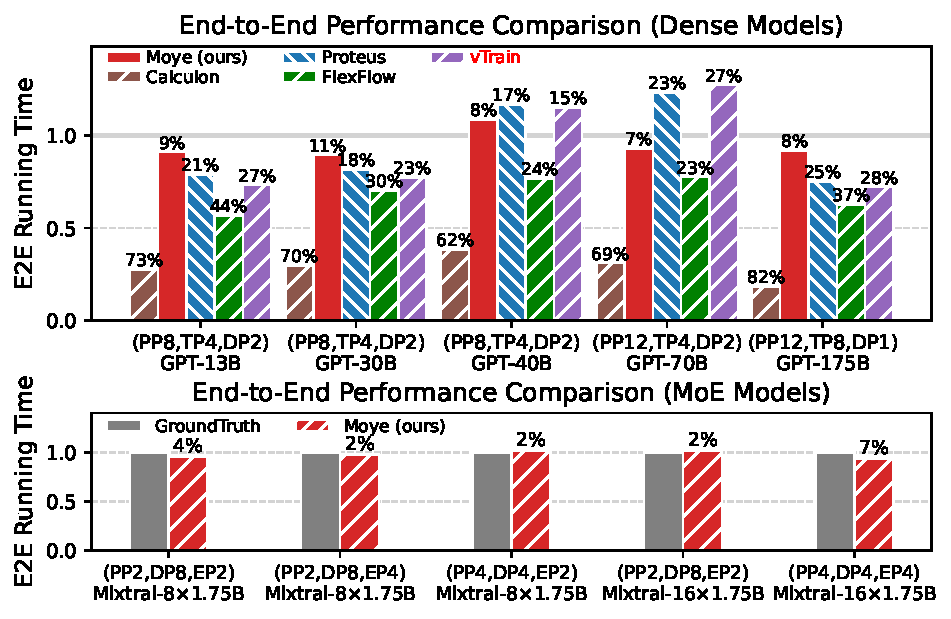
\includegraphics[width=1\linewidth]{figures/evaluation/NEW_end_to_end_normalized.pdf}
    \caption{\yc{End-to-end training step time comparison on dense and MoE models (up to 96 H800 GPUs). 
    All results are normalized to ground truth ($y{=}1.0$/gray bars). 
    Numbers above bars denote prediction error. Baseline systems do not support MoE simulation.}}
    \vspace{-0.2em}
    \label{fig:end_to_end} 
\end{figure}

\noindent\textbf{Accuracy.} 
We evaluate the end-to-end accuracy of \sys on H800 clusters of varying scales using Megatron-LM. 
As shown in Figure~\ref{fig:end_to_end}, \sys consistently achieves high fidelity across diverse parallelism configurations. 
For 96-GPU scenarios, the prediction error is 7\% for GPT-70B ($12\times4 \times2$) and 8\% for GPT-175B ($12\times8\times1$). 
In contrast, baseline simulators deviate significantly: Proteus and FlexFlow show errors exceeding 25\%, while Calculon is overly optimistic (error $>$69\%) due to its reliance on ideal analytical models. 
\sys also attains high accuracy on MoE models, with an average error of 3.4\%. 
Across models, \sys achieves average errors of 4.5\% and 17.8\% for computation and communication operations. 
Its accuracy is further improved by modeling slowdown from overlapping kernels. 
In our settings here, computation--communication overlap accounts for 6.0\%--9.8\% of total step time, and simulating the overlap-induced slowdown improves end-to-end accuracy by 3.6\%--5.2\%. 
As training systems increasingly optimize for aggressive overlap \cite{deepep}, accurate slowdown prediction may become even more critical.
\yc{
\begin{figure}[t]
    \centering
    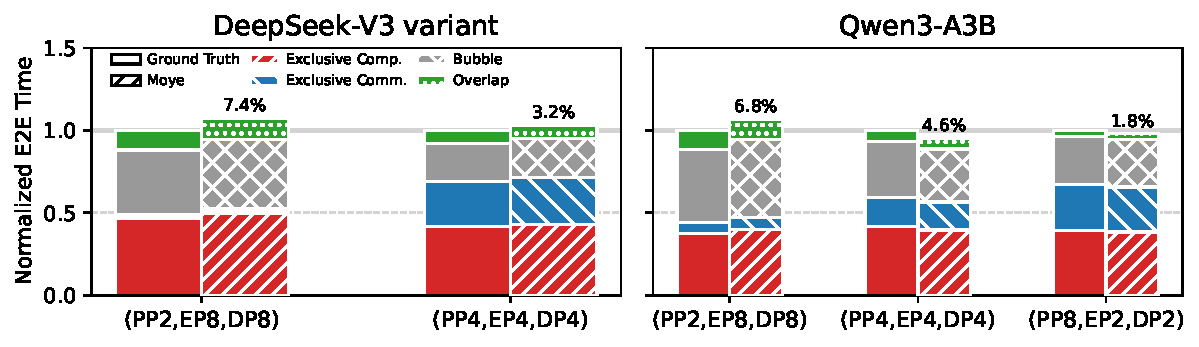
\includegraphics[width=1\linewidth]{figures/evaluation/latest_models_e2e_breakdown.pdf}
    \caption{\yc{End-to-end component breakdown for two latest MoE models in our H800 setup. Left: DeepSeek-V3 variant. Right: Qwen3-A3B. Each configuration shows a textured ground-truth bar and a colored stacked \sys bar decomposed into exclusive computation, exclusive communication, bubble, and overlap. Numbers above \sys bars denote absolute end-to-end prediction error. Proteus, FlexFlow, and Calculon are omitted because they do not support these latest models.}}
    \label{fig:end_to_end_latest_models}
\end{figure}

\noindent\textbf{Latest MoE models.}
We further evaluate \sys on two recently released MoE models, DeepSeek-V3 variant and Qwen3-A3B, in our H800 setup. These two models stress different MoE execution paths rather than merely larger parameter counts: Qwen3-A3B increases routing fan-out and expert diversity, whereas the DeepSeek-V3 variant combines MLA, group-limited routing, shared experts, and all-to-all expert communication. As shown in Figure~\ref{fig:end_to_end_latest_models}, other SOTA simulators cannot simulate these latest models, so we only compare \sys against ground truth. Across the five feasible configurations, \sys achieves an average end-to-end prediction error of 4.8\%, with a maximum error of 7.4\%. For Qwen3-A3B, the error ranges from 1.8\% to 6.8\%; for DeepSeek-V3 variant, it ranges from 3.2\% to 7.4\%. The overlap portion spans 3.5\%--12.8\% of total step time, while bubble remains a major contributor at 24.0\%--47.3\%. This breakdown indicates that the remaining gap is not dominated by expert communication alone, but also by compute-side phases and their interaction with overlap and pipeline bubbles.

\begin{table}[t]
\centering
\small
\renewcommand{\arraystretch}{0.95}
\begin{tabular}{@{}lcccc@{}}
\toprule
\textbf{Skew} & \textbf{Load} & \textbf{GT straggler} & \textbf{\sys straggler} & \textbf{Proxy err.} \\
\midrule
Balanced & 1.00 & 1.04 & 1.24 & 7.88\% \\
Moderate & 1.54 & 1.02 & 1.08 & 4.40\% \\
Strong & 3.00 & 1.08 & 1.22 & 6.64\% \\
\bottomrule
\end{tabular}
\caption{\yc{Controlled routing-skew stress test on the DeepSeek-V3 variant in our 8-GPU A800 setup ($PP{=}2$, $TP{=}1$, $EP{=}4$, $DP{=}4$), along the widely used no-token-dropping path. Load reports the hottest-to-median expert token count. The strongest skew regime increases the GT straggler ratio from the near-balanced 1.02--1.04 range to 1.08, while \sys keeps the critical-path proxy error within 4.4\%--7.9\%.}}
\label{table:moe_routing_skew}
\end{table}

\noindent\textbf{MoE routing-skew sensitivity.}
We further stress the DeepSeek-V3 variant with controlled expert-load skew while keeping the model architecture and parallel configuration fixed along the widely used no-token-dropping path. The moderate-skew case remains close to the balanced setting within system noise, but the strong-skew case makes a subset of EP ranks dominate the critical path more clearly. \sys predicts this stressed regime with 6.64\% critical-path proxy error, showing that its MoE fidelity extends beyond near-balanced routing under controlled routing skew. Explicit capacity-factor extremes and token-dropping/capacity-aware admission control remain future work.
}


\yc{
\begin{figure}[t]
    \centering
    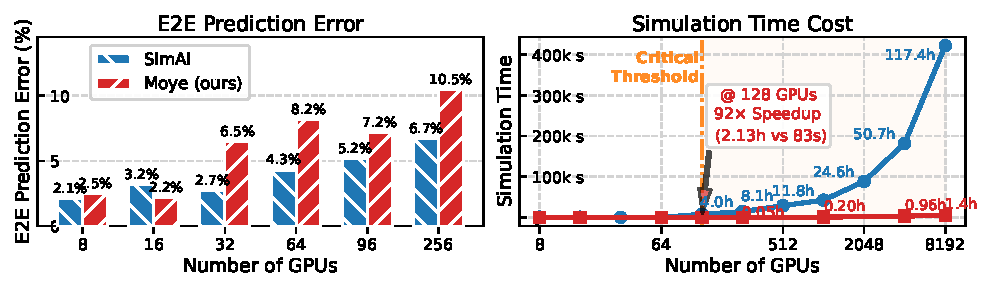
\includegraphics[width=1\linewidth]{figures/evaluation/simai_vs_moye.pdf}
    \caption{\yc{Comparison of \sys and SimAI on GPT-175B (H800 cluster, 3D parallelism). 
    Left: end-to-end prediction error across cluster scales. 
    Right: simulation time cost (log-log scale). 
    Beyond 128 GPUs, \sys achieves a 91.8$\times$ speedup over SimAI while maintaining comparable accuracy.}}
    \label{fig:simai_vs_moye}
    \vspace{-1em}
\end{figure}

\noindent\textbf{Comparison with packet-level simulator.}
We compare \sys against SimAI~\cite{SimAI2025NSDI}, a packet-level network simulator built on ns-3, on GPT-175B training across 8--8{,}192 H800 GPUs (Figure~\ref{fig:simai_vs_moye}).
In terms of accuracy, both simulators achieve comparable end-to-end prediction errors at small scales (2--3\% at 8--32 GPUs).
As the cluster grows, \sys's error increases moderately to 10.5\% at 256 GPUs, while SimAI remains at 6.7\%---a gap attributable to SimAI's finer-grained packet-level communication modeling.
However, the simulation time gap is dramatic.
At 128 GPUs, \sys completes in 83 seconds---a 91.8$\times$ speedup over SimAI's 7{,}655 seconds.
This advantage widens further at scale: at 8{,}192 GPUs, \sys finishes in 1.4 hours while SimAI requires over 117 hours.
For a design-space exploration sweeping 100 configurations on an 8{,}192-GPU cluster, \sys would complete in under 6 days, whereas SimAI would require over 1.5 years.
These results demonstrate that \sys offers a compelling accuracy--efficiency trade-off, making it practical for iterative what-if analysis at datacenter scale where packet-level simulation is prohibitively expensive.
}




% Ablation study
\yc{
\begin{figure}[t]
    \centering
    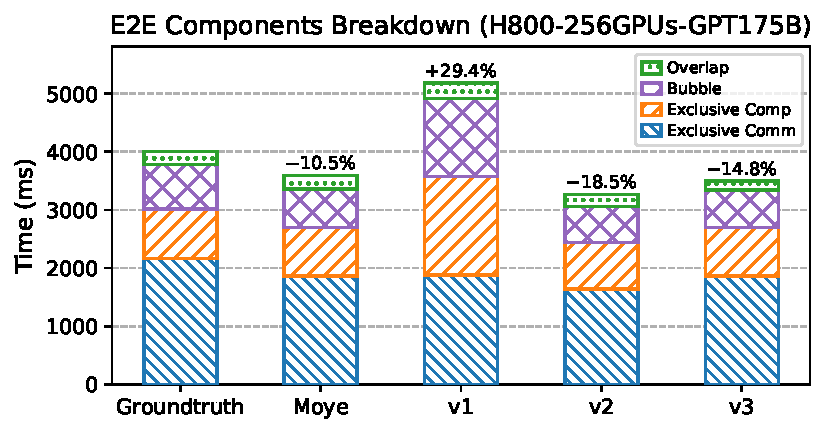
\includegraphics[width=0.75\linewidth]{figures/evaluation/component_breakdown_256gpu.pdf}
    \caption{\yc{Component breakdown of GPT-175B training step time on 256 H800 GPUs with 3D parallelism. Each bar decomposes the step time into exclusive computation, exclusive communication, bubble, and overlap. Numbers above bars denote end-to-end prediction error.}}
    \label{fig:ablation_breakdown}
    % \vspace{-1em}
\end{figure}

\noindent\textbf{Ablation study.}
To isolate the contribution of each key module, we perform an ablation study on GPT-175B (FP16) trained on a 256-GPU H800 cluster with 3D parallelism ($\text{PP}=16, \text{TP}=8, \text{DP}=2$).
We disable one module at a time and report the signed prediction error for each time component against ground truth (Figure~\ref{fig:ablation_breakdown} and Table~\ref{table:ablation}).

\begin{table}[t]
\centering
\small
\renewcommand{\arraystretch}{0.9}
\resizebox{\columnwidth}{!}{
\begin{tabular}{@{}lrrrrr@{}}
\toprule
\textbf{Variant} & \textbf{Excl. Comp.} & \textbf{Excl. Comm.} & \textbf{Bubble} & \textbf{Overlap} & \textbf{End-to-End} \\
\midrule
\sys (Full)            & $-$2.2\%   & $-$14.0\%  & $-$13.2\%  & $+$1.1\%   & $-$10.5\% \\
w/o Ex-situ Tracer (v1)   & $+$98.2\% & $-$13.0\%  & $+$75.0\%  & $+$21.1\%   & $+$29.4\% \\
w/o White-box Comm. (v2)    & $-$6.3\%   & $-$24.4\%  & $-$19.0\%  & $-$6.8\%   & $-$18.5\% \\
w/o Slowdown Pred. (v3)     & $-$2.5\%   & $-$13.9\%  & $-$15.7\%  & $-$31.9\%  & $-$14.8\% \\
\bottomrule
\end{tabular}}
\caption{\yc{Ablation study on GPT-175B (256 H800 GPUs, 3D parallelism). Each column shows the signed prediction error of the corresponding time component relative to ground truth.}}
\label{table:ablation}
\vspace{-1em}
\end{table}

Removing the ex-situ computation profiler and substituting analytical FLOPS estimates inflates the exclusive computation error to $+$98.2\%, which cascades into $+$75.0\% bubble error and $+$29.4\% end-to-end deviation---the largest among all variants.
Replacing the white-box communication model with an $\alpha$-$\beta$ model increases the exclusive communication error from 14.0\% to 24.4\% and worsens end-to-end accuracy from 10.5\% to 18.5\%.
Disabling slowdown prediction degrades overlap estimation from $+$1.1\% to $-$31.9\% error, raising the end-to-end error by 4.3 percentage points.
These results confirm that all three modules contribute meaningfully to \sys's end-to-end fidelity.
}



\yc{
\noindent\textbf{Simulation cost.}
We investigate \sys's two time costs:
(1) profiling time cost, and
(2) simulation time cost, including initialization and execution, and excludes the one-time, reusable workload tracing cost. 
}
As detailed in Table~\ref{table:simulation_cost}, \sys is highly efficient across training scenarios. For DDP, simulation is consistently fast, averaging about 10 seconds. The advantage is more pronounced for complex 3D parallelism; by leveraging its white-box communication model, \sys simulates a 128-GPU setup in 83 seconds—a 91.8x speedup over packet-level simulators like SimAI (7655s). This efficiency scales to large configurations, enabling the simulation of one step of an 8,192-GPU cluster in $<$1.4 hours.
For a typical design-space exploration over 100 training configurations on such a system, \sys would complete all simulations in under 6 days.
At this scale, the much higher per-configuration cost of packet-level network simulation (like SimAI) would push turnaround time to 1.5 years.



% table1
\begin{table}[t]
\centering
\small
\renewcommand{\arraystretch}{0.8}
\resizebox{\linewidth}{!}{
\begin{tabular}{ccccccccc}
\toprule
\multirow{2}{*}{\#GPUs} & \multicolumn{4}{c}{\textbf{VGG19}} & \multicolumn{4}{c}{\textbf{GPT 13B$\sim$175B}} \\ \cmidrule(lr){2-5} \cmidrule(lr){6-9}
                        & \textbf{Init.} & \textbf{Execution} & \textbf{Sim. Total} & \textbf{Trace} & \textbf{Init.} & \textbf{Execution} & \textbf{Sim. Total} & \textbf{Trace} \\ \midrule
256                     & 0.4            & 10.3           & 10.7           & \yc{18.2}      & 8.4             & 159.2          & 167.6          & \yc{1350.2}           \\
1024                    & 0.3            & 9.7            & 10.0           & \yc{18.5}      & 35.9            & 682.8          & 718.7          & \yc{1926.7}           \\
4096                    & 0.4            & 10.2           & 10.6           & \yc{17.8}      & 149.9           & 3307.8         & 3457.7         & \yc{2688.3}           \\
8192                    & 0.3            & 10.3           & 10.5           & \yc{18.3}      & 374.7           & 4602.2         & 4976.9         & \yc{3498.2}           \\ \bottomrule
\end{tabular}}
\caption{\yc{The simulation time costs of \sys in seconds. VGG19 is trained using the DDP mode, while GPT models (ranging from 13B to 175B) are trained using 3D parallelism.}}
\label{table:simulation_cost_old}
% \vspace{-2em}
\end{table}




\subsection{Computation and Memory Usage Simulation}
\label{subsec:workload_perf}

\noindent We evaluate \sys's accuracy in simulating computation workloads on both H800 and A800 clusters, using VGG19 (with DeepSpeed), GPT-13B and Mixtral-8×1.75B (both with Megatron-LM) under various PP/EP configurations. 

\noindent\textbf{Accuracy.} \sys reconstructs the computation workload by tracing all computational \ops and reproducing their execution sequence based on the \wg. Per-GPU \op running times are derived through \sys's \extractor without requiring a full-scale deployment. 
As shown in Figure~\ref{fig:comp_h}, \sys achieves a maximum overall error of 8.31\%. In contrast, while \bs and \ff maintain relatively low error rates for VGG19 under DeepSpeed (8.6\% and 17.81\%, respectively), their errors escalate dramatically for GPT-13B under Megatron-LM, reaching 91.53\% and 109.14\%, respectively.
The root cause of this discrepancy is that Proteus and FlexFlow rely heavily on standard PyTorch \ops, failing to incorporate the custom fused \ops that frameworks like Megatron-LM employ for performance optimization. 
Such specialized \ops cannot be accurately modeled without extracting their runtime characteristics directly from the target training framework (as we disccusion in~\cref{sec:motivation}). 
Calculon overestimates computation time in an overly idealized manner (error rate $>400\%$), because its modeling relies on hardware's analytical FLOPS values, which severely deviate from real hardware execution.
By precisely tracing, \sys captures the actual \op behaviors and achieves substantially higher accuracy.

\begin{figure}[t] 
    \centering 
    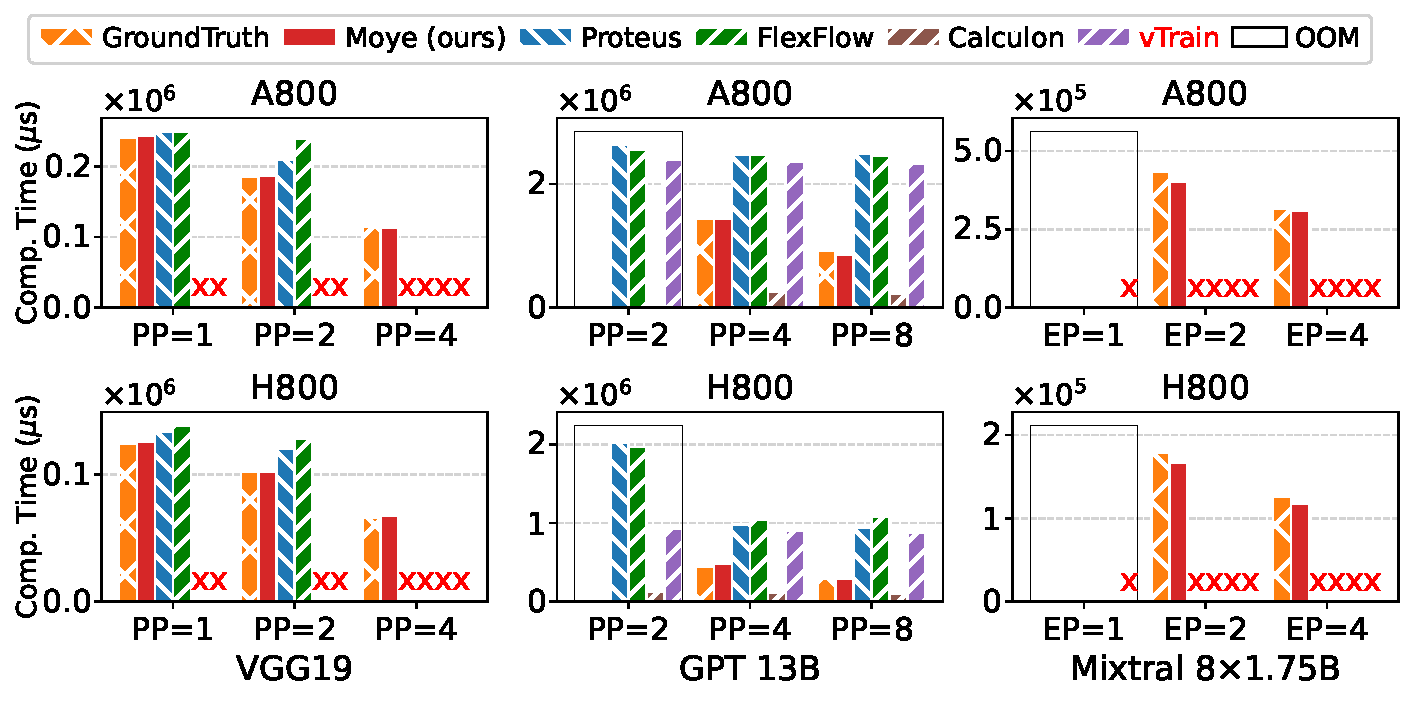
\includegraphics[width=1\linewidth]{figures/evaluation/comp_h800_a800_with_vtrain.pdf} 
    \caption{\yc{
        Computation times of various workloads on A800 and H800 clusters under different parallelization settings. Crosses denote cases not supported by the baselines, while squares mark configurations that encountered OOM errors during real execution.
    }}
    \label{fig:comp_h}
    \vspace{-2.2mm}
\end{figure}

\begin{figure}[t] 
    \centering 
    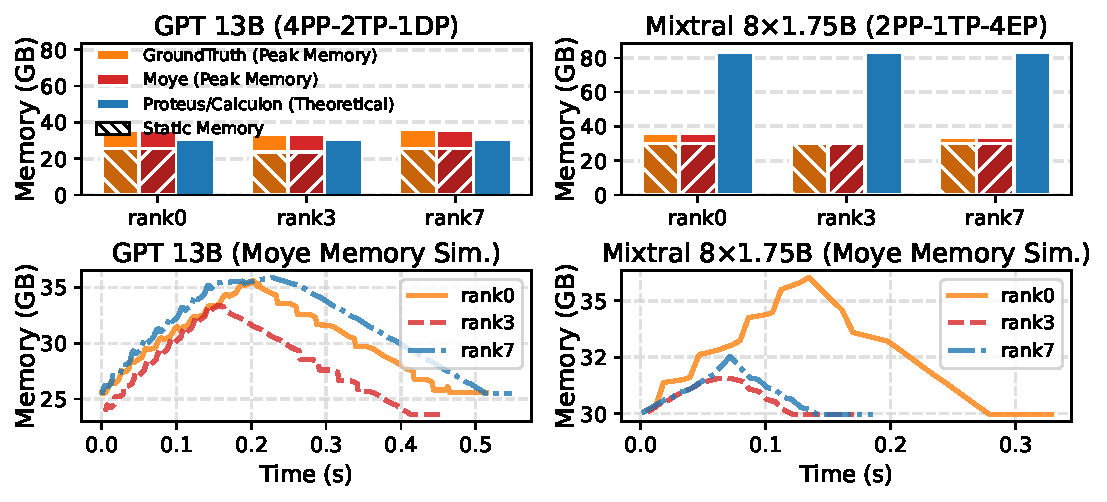
\includegraphics[width=1\linewidth]{figures/evaluation/memory_analysis_final.pdf} 
    \vspace{-2em}
    \caption{
        Validation of Moye's GPU memory simulation for GPT-13B and Mixtral-8$\times$1.75B on our 8-GPU A800 cluster (8 ranks), showing three representative ranks.
        It demonstrates Moye's ability to capture dynamic per-rank memory usage within a training step (excluding communication time). We set num\_micro\_batch=micro\_batch\_size=1 here.
    }
    \label{fig:memory}
    \vspace{-3mm}
\end{figure}

\vspace{0.1em}
\noindent\textbf{Generality.}
\sys is the only high-fidelity simulator that supports MoE workloads (error $<6\%$, Figure~\ref{fig:comp_h}). 
None of the baselines can handle MoE models.
Even for CNNs, Proteus and FlexFlow fail on certain configurations (e.g., VGG19 at PP=4) due to their reliance on manual, pre-hardcoded workload construction. 
In contrast, \sys supports simulations across a wide range of training design spaces. 
We further demonstrate its scalability via an ex-situ simulation of 8,192 GPUs in \cref{sec:usecase}.

\vspace{0.1em}
\noindent\textbf{GPU Memory usage.}
\sys supports high-fidelity GPU memory usage simulation through ex-situ profiling.
Figure~\ref{fig:memory} (upper) shows the peak memory usage (including both static and dynamic components), where \sys achieves nearly 100\% accuracy on GPT-13B and Mixtral-8$\times$1.75B for different ranks.
In contrast, analytical methods can result in 18.0\% error for GPT-13B, and for MoE models (Mixtral-8$\times$1.75B), the error even increase to 2.58$\times$ (a gap of 51 GB).
\sys can also reflect dynamic GPU allocation behavior during training, as shown in Figure~\ref{fig:memory} (lower)—a capability absent in existing simulators.
We believe this ability can help engineers identify potential optimization opportunities.

\begin{figure}[t] 
    \centering 
    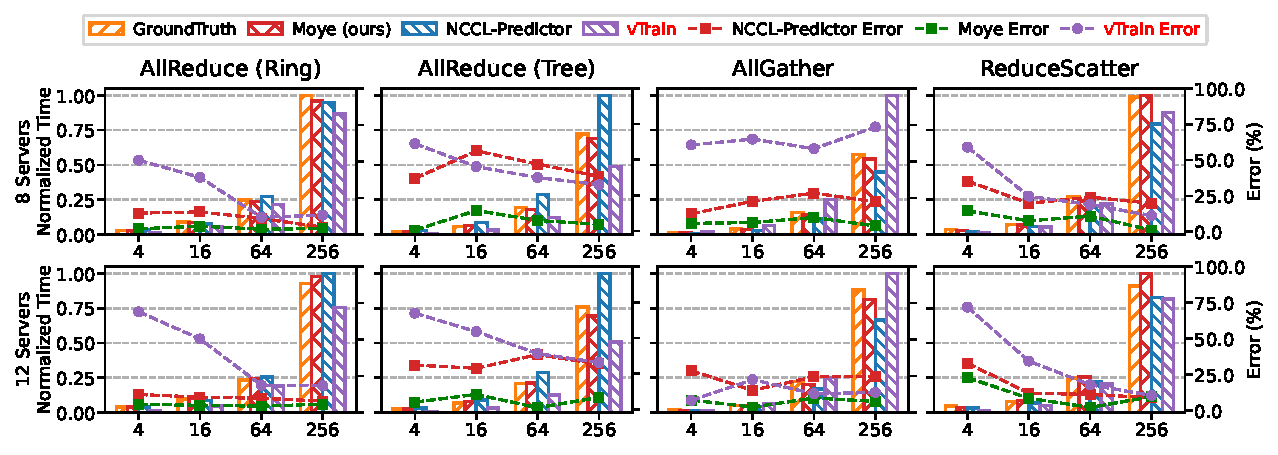
\includegraphics[width=1\linewidth]{figures/evaluation/inter_nccl.pdf} 
    \vspace{-.5cm}
    \caption{\yc{Running time and prediction error for inter-server CC kernels on H800 GPUs across varying tensor sizes and cluster scales. Each subplot is normalized relative to the operation with the longest running time.}}
    \label{fig:inter_nccl}
    \vspace{-1.2em}
\end{figure}

\subsection{Communication Simulation}
\label{subsec:allreduce_perf}

\noindent We now evaluate the effectiveness of \sys's communication simulation, comparing it against NCCL-Predictor~\cite{nccl}, the underlying communication model used by both \bs and \ff. NCCL-Predictor leverages parameters tuned from production experience and employs an ${\alpha-\beta}$ model~(\cref{subsec:challenges}).

\noindent\textbf{Accuracy.}  
Figures~\ref{fig:inter_nccl} show the prediction accuracy of collective communication across message sizes (4MB-256MB) and cluster scales. 
\sys consistently outperforms NCCL-Predictor, with average errors of 12.6\% and 13.8\% on 8- and 12-server H800 clusters, improving upon NCCL-Predictor by 29.6\% and 19.4\%, respectively.
\fx{Here, for 8- and 12-server clusters we set the scaling factor $c_{\mathrm{scale}}(N)$ to 1.023 and 1.063, respectively.}
The gap is smallest on ring-based \ar (4.2\%), where NCCL's heavy optimizations align well with the ${\alpha-\beta}$ model. 
For other patterns---especially tree-based \ar---\sys achieves much higher accuracy, reducing errors by up to 33.5\%.  

These improvements stem from \sys's profiling-based white-box model, which captures bandwidth utilization and synchronization overheads that NCCL-Predictor's simplified assumptions overlook. 
As a result, \sys maintains consistent accuracy for both small and large messages, whereas NCCL-Predictor suffers average errors of 27.6\% on 4MB and 16MB inputs.  
Finally, \sys's white-box design also accelerates simulation speed, as shown in~\cref{subsec:overall_perf}.
\yc{We further evaluate \sys on the \texttt{all-to-all}. As shown in Figure~\ref{fig:alltoall_error}, \sys achieves an average error of 13.6\% across 1- and 2-server H800 configurations, compared to 25.8\% for the $\alpha$-$\beta$ model. Since expert dispatch/combine in our Qwen3-A3B and DeepSeek-V3-style workloads is instantiated as \texttt{all-to-all}, this result directly validates \sys's communication model on the dominant MoE-specific collective, rather than only on dense-model traffic.}

\begin{figure}[t]
    \centering
    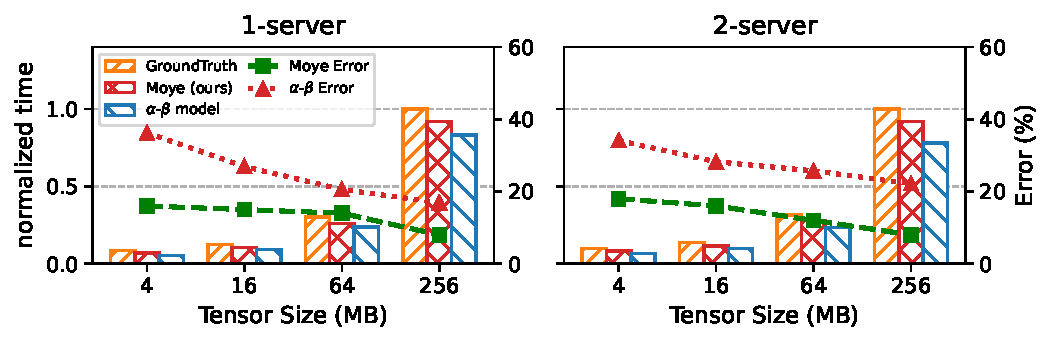
\includegraphics[width=.75\columnwidth]{figures/evaluation/alltoall_error_compare.pdf}
    \vspace{-0.6em}
    \caption{\yc{\sys's all-to-all running time prediction on H800 clusters.}}
    \label{fig:alltoall_error}
    % \vspace{-1em}
\end{figure}

\begin{table}[t] 
    \centering
    \small
    \renewcommand{\arraystretch}{0.8}
    \resizebox{\columnwidth}{!}{ 
        \begin{tabular}{@{}llllllll@{}}
            \toprule
            Tensor size (MB)           & 4      & 8       & 16    & 32      & 64      & 128     & 256     \\
            Chunk size ($10^3$ bytes)  & 18     & 36      & 72    & 72      & 72      & 144     & 288     \\ \midrule
            \begin{tabular}[c]{@{}l@{}}Intra-server \\ Round trip ($\mu$s) \end{tabular} & 57.43  & 64.36  & 73.62 & 74.61   & 77.46   & 75.55   & 99.23   \\ \midrule
            \begin{tabular}[c]{@{}l@{}}Inter-server \\ Round trip ($\mu$s) \end{tabular} & 54.3   & 72.32  & 106.73 & 112.9   & 111.25  & 174.2   & 278.98  \\ \midrule
            Reduce operation ($\mu$s) & 50.14  & 65.86  & 102.46 & 219.89  & 463.43  & 841.71  & 1657.72 \\ \bottomrule
        \end{tabular}}
    \caption{The breakdown of \sys's \ar running time, profiled in the H800 cluster using 32 GPUs.}
    \vspace{-4mm}
    \label{table:allreduce_param}
\end{table}

\noindent\textbf{Breakdown analysis.}
Table~\ref{table:allreduce_param} reports the breakdown of \ar runtime on a 32-GPU H800 cluster, separating intra-server latency, inter-server latency, and reduction computation across tensor sizes. 
Intra-server round-trip time increases moderately with tensor size (57.4~\textmu s at 4MB to 99.2~\textmu s at 256MB), reflecting the overhead of scheduling more thread blocks for larger chunks. 
Inter-server round-trip time shows a similar trend, growing to 279~\textmu s at 256MB. 
Reduction computation dominates at large tensors, scaling nearly linearly from 50.1~\textmu s (4MB) to 1658~\textmu s (256MB). 
These results demonstrate that \sys accurately captures both communication and computation overheads across varying message sizes. 




\subsection{Slowdown Prediction} 
\label{subsec:interference_perf}

\begin{figure}[t]
    \centering 
    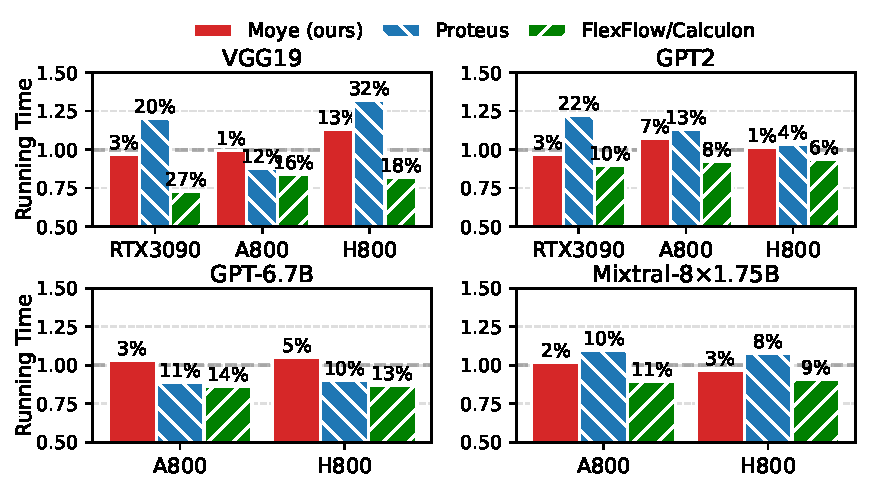
\includegraphics[width=0.95\linewidth]{figures/evaluation/model_wise_overlap_normolized2.pdf} 
    \vspace{-1em}
    \caption{
        Normalized model-wise computation time on H800, A800, and RTX3090 GPUs. 
        \sys (prediction-based) is compared against Proteus (fixed-parameter slowdown modeling) and FlexFlow/Calculon (no slowdown modeling). 
        Numbers above bars denote prediction error relative to ground truth (gray line at $y{=}1.0$).
    }
    \label{fig:model_wise_overlap}
\end{figure}

\begin{table}[t]
    \centering
    \small
    \renewcommand{\arraystretch}{0.85}
    \resizebox{0.85\columnwidth}{!}{
        \begin{tabular}{@{}llcccc@{}}
        \toprule
        Solution        & GPU & 5\% Error & 10\% Error & 15\% Error & RMSE \\ \midrule
        \sys     & \multirow{2}{*}{\centering 3090} & 61.48\% & 73.62\% & 76.52\% & 1.0935 \\
        Proteus         &                                   & 8.52\%  & 13.62\% & 19.28\% & 1.4953 \\ \midrule
        \sys      & \multirow{2}{*}{\centering A800}  & 61.03\% & 69.82\% & 75.01\% & 0.7147 \\
        Proteus         &                                   & 59.04\% & 65.45\% & 70.51\% & 1.5170 \\ \midrule
        \sys     & \multirow{2}{*}{\centering H800}  & 43.18\% & 51.59\% & 57.73\% & 0.5626 \\
        Proteus         &                                   & 34.78\% & 37.36\% & 40.18\% & 1.5493 \\ \bottomrule
        \end{tabular}}
    \caption{Fraction of cases where the slowdown prediction error is within the given error range.}
    \label{table:performance_comparison}
    \vspace{-1em}
\end{table}

\noindent Most simulators overlook the performance slowdown caused by kernel overlap. We compare \sys with \bs, the only baseline known to model this effect, which does so using a simple heuristic based on GPU architecture and model type.

\noindent\textbf{Prediction accuracy.}  
We evaluate slowdown prediction on $\sim$10,000 kernels (Table~\ref{table:performance_comparison}). 
\sys consistently outperforms the baseline heuristic, especially on data-center GPUs. 
On the H800, 57.7\% of predictions fall within 15\% error, compared to 40.2\% for the baseline, and the RMSE is nearly 3$\times$ lower (0.56 vs.\ 1.55). 
Similar gains hold on the A800, while on consumer-grade RTX 3090 GPUs, \sys again shows substantially lower error across all metrics. 

\noindent\textbf{Model-wise evaluation.} 
We further evaluate the impact of slowdown-aware modeling on training simulation accuracy across representative models. 
Experiments are conducted on modern training setups that already incorporate computation--communication overlapping: VGG19 and GPT2 with PyTorch DDP, GPT-6.7B with Megatron-LM 3D parallelism, and Mixtral-8$\times$1.75B with Flux, which enables fine-grained GroupedGEMM overlap. 
We slightly adjust model parameters so that overlapped kernels account for more than 25\% of execution time in all cases. 
Compared to baselines that ignore slowdown effects (FlexFlow and Calculon), incorporating slowdown improves the accuracy of simulating the computation portion by about 4\% on average. 
At the model level, \sys achieves the lowest prediction error across all tested architectures: 2--5\% on average, compared to 8--23\% for Proteus and 10--37\% for FlexFlow/Calculon (Figure~\ref{fig:model_wise_overlap}). 
These results highlight that accurate slowdown prediction is essential for faithfully modeling modern training workloads with heavy overlap. 

%!TEX root = main.tex

\section{Use Case Study} 
\label{sec:usecase}

\begin{figure}[t] 
    \centering 
    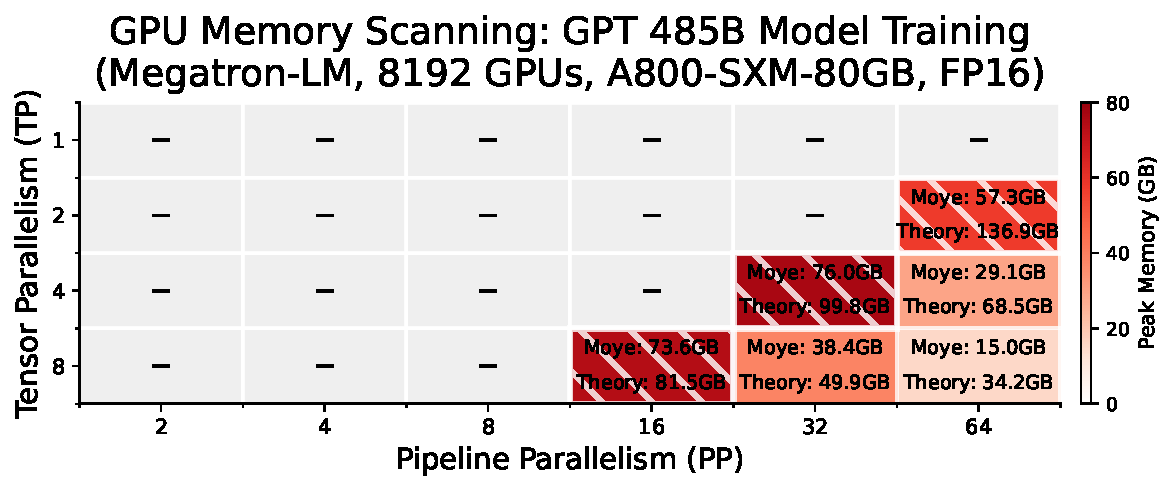
\includegraphics[width=1\linewidth]{figures/evaluation/memory_heatmap_485B_academic.pdf} 
    \vspace{-5mm}
    \caption{GPU memory constraint scanning for a 485B model on 8192 GPUs. Each cell represents a unique parallelism strategy defined by its PP and TP sizes, with DP implicitly set to satisfy PP * TP * DP = 8192. Gray cells indicate OOM conditions. The red, hatched cells highlight configurations that are empirically feasible yet are incorrectly identified as OOM by baseline analytical models.}
    \label{fig:memory_heatmap} 
    \vspace{-1em}
\end{figure}


\subsection{Use Case: Training Strategy Search} 
\label{sec:training-strategy-search}
\noindent A recurring practical question in large-scale training is: given a GPU cluster and the LLM, how should the training job and the parallelisms be configured to achieve the best efficiency? Answering this question by trial-and-error on the real cluster is prohibitively expensive, as each trial may waste thousands of GPU-hours. 
\sys provides a low-cost alternative by efficiently searching across a wide range of parallelism and system configurations. 

The workflow proceeds in two stages. 
First, \sys conducts a GPU memory feasibility scan via grid search over parallelism choices (see Figure~\ref{fig:memory_heatmap}). 
This step leverages its high-fidelity memory simulation to filter out infeasible configurations and avoid false OOM predictions that plague existing analytical models (e.g., Proteus, Calculon). 
Second, for all surviving candidates, \sys performs end-to-end simulation to estimate throughput and cost. 
By faithfully reconstructing the interaction between computation, communication, and memory behaviors, \sys enables accurate evaluation of training efficiency under each configuration. 
From these results, \sys recommends the configuration that minimizes time-to-train and monetary cost (see Table~\ref{tab:perf_time_cost_analysis}).




\begin{table}
    \centering
    \small
    \resizebox{0.48\textwidth}{!}{%
        \begin{tabular}{lcccc}
            \toprule
            \textbf{Setting} & \textbf{Peak memory} & \textbf{Throughput} & \textbf{Time (days)} & \textbf{Cost} \\
            \midrule
            \rowcolor{red!25}
            (PP16, TP8, DP64) & 73.6 GB & 455.8k tokens/s & 12.7 & \$2.45M \\
            \rowcolor{gray!25}
            (PP32, TP8, DP32) & 38.4 GB & 361.1k tokens/s & 16.0 & \$3.09M \\
            (PP64, TP8, DP16) & 15.0 GB & 331.9k tokens/s & 17.4 & \$3.36M \\
            (PP32, TP4, DP64) & 76.0 GB & 350.0k tokens/s & 16.5 & \$3.19M \\
            (PP64, TP4, DP32) & 29.1 GB & 222.1k tokens/s & 26.1 & \$5.02M \\
            (PP64, TP2, DP64) & 57.3 GB & 308.3k tokens/s & 18.8 & \$3.62M \\
            \bottomrule
        \end{tabular}
    } 
    \caption{Simulation results under different training configurations on 8,192 A800 GPUs for GPT 485B with a volume of 500B tokens. The training time is calculated using the total volume and predicted throughput, and the cost is derived accordingly using the market rent price of A800. The red row denotes \sys's choice, while the gray row is Calculon's choice which is suboptimal.}
    \label{tab:perf_time_cost_analysis}
    \vspace{-1.5em}
\end{table}


\yc{
\subsection{Use Case: Scaling-up Analysis} 
\label{sec:scale-up}
\begin{figure}[t]
    \centering
    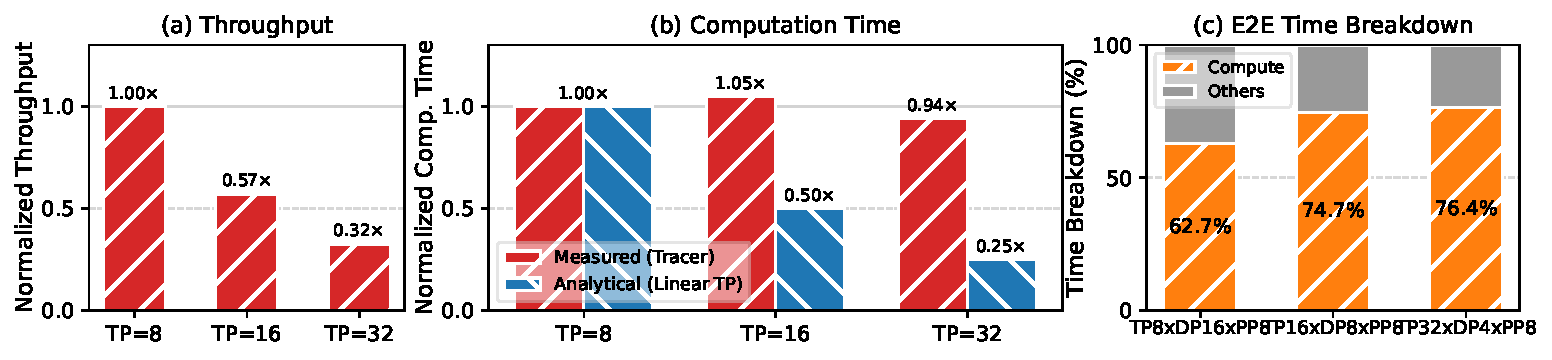
\includegraphics[width=1\linewidth]{figures/evaluation/tp_scaling_gpt175b_world1024.pdf}
    \vspace{-6mm}
    \caption{\yc{Scaling-up analysis for GPT-175B on 1,024 GPUs (fixed PP=8 and global batch size 256). \textbf{(a)} Normalized throughput under different TP degrees. \textbf{(b)} Normalized per-microbatch computation time from \sys's framework-specific ex-situ tracer versus an analytical model assuming ideal linear TP scaling. \textbf{(c)} Stage0 time breakdown into computation and \textit{others} across TP$\times$DP$\times$PP configurations.}}
    \label{fig:tp_scaling_gpt175b_world1024}
    \vspace{-1em}
\end{figure}

\noindent\textbf{Larger TP does not improve E2E throughput.}
A natural expectation is that scaling up TP to match more GPUs within a node can exploit fast NVLink/NVSwitch links and accelerate model-shard execution. We test this intuition on GPT-175B with 1,024 GPUs, fixed PP=8, and global batch size 256. Figure~\ref{fig:tp_scaling_gpt175b_world1024}(a) shows the opposite trend: normalized throughput drops from 1.0 at TP=8 to 0.57 and 0.32 at TP=16 and TP=32, corresponding to iteration time increasing from 34.4\,s to 60.5\,s and 106.2\,s. Thus, simply enlarging the TP domain can hurt rather than help end-to-end efficiency.

\noindent\textbf{Why it happens: TP increases, DP shrinks, but per-microbatch compute does not.}
Under fixed world size and PP, increasing TP compresses DP from 16 to 8 to 4, which increases the number of micro-batches per iteration from 16 to 32 to 64. This trade-off would be acceptable only if each micro-batch became proportionally cheaper. However, Figure~\ref{fig:tp_scaling_gpt175b_world1024}(b) shows that \sys's tracer measures nearly flat per-microbatch computation time: 1,349.7\,ms, 1,412.1\,ms, and 1,267.2\,ms for TP=8/16/32. In contrast, a naive analytical model assuming ideal linear TP scaling predicts 1,349.7\,ms, 674.8\,ms, and 337.4\,ms. Because the expected compute speedup never materializes, total stage0 computation rises sharply from 21.6\,s to 45.2\,s and 81.1\,s, which directly drives the throughput collapse.

\noindent\textbf{Takeaway for scaling-up decisions.}
Figure~\ref{fig:tp_scaling_gpt175b_world1024}(c) confirms that computation dominates the bottleneck stage across TP8$\times$DP16$\times$PP8, TP16$\times$DP8$\times$PP8, and TP32$\times$DP4$\times$PP8: its share grows from 62.7\% to 74.7\% and 76.4\%, while \textit{others} remain non-trivial. Therefore, once memory feasibility is satisfied, TP should be treated as a tunable parameter rather than maximized by default; when larger TP only reduces DP and increases micro-batching, additional scale-up can reduce throughput. This use case highlights the value of \sys's high-fidelity tracing inputs for exposing non-ideal scaling and guiding reliable LLM training configuration decisions.
}
%!TEX root = main.tex 

\section{Limitations and Discussions} 
\label{sec:discussion}

\noindent\sys has limitations and we wish to improve it in at least the following directions.
\begin{comment}
\noindent\textbf{Computation prediction.}
\sys relies on trace-based profiling rather than purely architectural models. By extracting real execution traces from small-scale runs and extrapolating to large systems, \sys avoids the high inaccuracies (e.g., >70\%) we observed when using architecture-focused simulators like SCALE-sim~\cite{samajdar2018scale}. In the future, we plan to explore hybrid approaches that blend \sys's profiling accuracy with more flexible architectural models.
\end{comment}

\noindent\textbf{Communication prediction.}
% \sys's white-box modeling and offline profiling offer an accurate, low-overhead method for communication kernel estimation. 
\sys positions itself between hand-tuned $\alpha$--$\beta$ models and packet-level network simulators.
We plan to investigate learning based solutions like m3~\cite{li2024m3} that efficiently predicts flow-level performance while capturing network-centric factors such as transport protocols. 
% We also wish to extend our modeling to explicitly consider network topology and the potential bandwidth contention, which is currently missing.

\noindent\textbf{Parallelism.}
\sys does not support sequence/context parallelism currently.
We plan to integrate them in subsequent releases.

\noindent\textbf{MoE routing policies.}
Our current paired validation focuses on the widely used no-token-dropping path in Megatron-style MoE training and evaluates controlled routing skew as the primary source of expert-load imbalance. 
We leave explicit capacity-factor extremes, token-dropping/capacity-aware admission control, and their effects on step-time tails and straggler behavior to future work.


% \yc{TODO: We also provide the comparison with packet-level simulator SimAI for further discussion of trad-off between fidelity and simulation speed.}



% It is also very interesting to 


% communication predictor currently relies on the knowledge profiled on a four-server cluster. Conventionally, it is the minimum requirement to construct the cluster suitable for double binary tree-based all-reduce. It is feasible to lower the required number of servers and use two servers to imitate such cluster topology. However, since the knowledge can be profiled ahead-of-time and is mostly reusable, it does not affect the results of the simulation. We leave this potential improvement to future work so that the profiling cost can be further reduced.


% \noindent\textbf{Model parallelism.} In this work, we discuss the simulation of data-parallel distributed DNN, which is the primary practice in DNN training. Model parallelism~\cite{shoeybi2019megatron, huang2019gpipe, NHPS19}is adopted for DNN models that cannot fit into one GPU memory. Model-parallel distributed training does not change the problem nature but requires additional send and receive operations among devices to transmit intermediate output. Through pipelining, they are also overlapped with computation kernels. Our prediction model can be trained to learn the interference in this scenario as model parallelism does not change the problem nature.


%!TEX root = main.tex 

\section{Related Work}
\label{sec:related}

\noindent We discuss related work other than those covered in \cref{sec:motivation}.

\noindent\textbf{GPU simulation.}
GPU computation simulators like SCALE-sim~\cite{samajdar2018scale} and Accel-Sim~\cite{khairy2020accel} focus on instruction-level modeling, while other approaches~\cite{hu2022dpro,lu2023distsim,luo2022srifty,zhu2020daydream} rely on profiling or tracing to capture accurate \op execution times. \sys similarly adopts a trace-based methodology, but crucially does so without requiring a full-scale deployment.




\noindent\textbf{Network simulation.} 
% Tools like ASTRA-sim~\cite{won2023astra}, FlexFlow~\cite{jia2019beyond}, Proteus~\cite{duan2024proteus}, and NCCL-Predictor~\cite{nccl} rely on the ${\alpha-\beta}$ model~\cite{valiant1990bridging}, offering simplicity but often limited accuracy. 
Discrete event simulators like ns-3~\cite{riley2010ns} and OMNeT++~\cite{varga2019practical} are well-known to have high overheads due to their packet-level whole-stack simulation. Other than parallelization optimizations \cite{GCLL23,BZTW24}, recently learning based approach to predict packet-level or flow-level performance without simulating the whole stack~\cite{ZNKY21,li2024m3,YPCL22} has shown promising results.
As mentioned before, integrating them with \sys for training simulation is a promising direction for future work. 

\begin{comment}
\noindent\textbf{Concurrent execution.} 
Concurrent GPU execution is increasingly employed to improve utilization~\cite{jiang2024megascale,chen2024centauri,zhang2017poseidon}, but it often degrades computation kernel performance, as these kernels overlap primarily with memcpy or communication operations. While this slowdown is significant (\cref{subsec:challenges}), most simulators ignore it. Proteus~\cite{duan2024proteus} is the only known simulator that attempts to model such slowdown, but its heuristic factor—based solely on GPU architecture and model type—is too coarse to handle diverse, unseen workloads. In contrast, \sys uses an ML-based approach for more accurate and generalizable slowdown predictions.
\end{comment}

%!TEX root = main.tex 

\section{Conclusion}
We presented \sys, a high-fidelity simulator for large-scale distributed ML training that bridges critical gaps in existing approaches. 
\sys simulates without full-scale deployment using ex-situ workload tracing, estimates CC performance via white-box modeling, and accounts for the slowdown caused by kernel overlapping.
Our evaluation shows that \sys not only achieves up to 3x lower simulation error than state-of-the-art baselines but also is highly efficient and practical.
We plan to open source \sys to the community.  
% By balancing accuracy, efficiency, and scalability, \sys sets a new standard for simulating large-scale training workloads at scale.


% \section*{Acknowledgment}
% Acknowledgments removed for blind review
\balance
\bibliographystyle{IEEEtran}
\bibliography{reference}

\end{document}

